%Kompiliuoti su XeLaTeX ir BibTeX

\documentclass[a4paper, 12pt, oneside]{article}

\usepackage[yyyymmdd]{datetime}

\usepackage{fontspec}
\usepackage{fontenc}
\usepackage{ulem}
\usepackage{cite}
\usepackage{mathtools}
\usepackage{amsmath}
\usepackage{amssymb}
%\usepackage{float}
\usepackage{graphicx}
\usepackage{multirow}
\usepackage[hyphens]{url}
\usepackage{caption}
\usepackage{subcaption}
\usepackage[svgnames]{xcolor}
\usepackage{lineno}
\usepackage[lithuanian]{babel}
\usepackage{hyperref}
\usepackage{siunitx}
\usepackage{floatrow}
\usepackage{indentfirst}
%\usepackage[parfill]{parskip}

\floatsetup[table]{capposition=top}

\hypersetup{breaklinks=true}
\urlstyle{same}

\usepackage{geometry}
\pagestyle{myheadings}
\geometry{
	left=3cm,
	right=1cm,
	top=2cm,
	bottom=2cm,
}
\pagenumbering{arabic}
\linespread{1.25}

\graphicspath{ {images/} }

\renewcommand{\dateseparator}{-}
\addto\captionslithuanian{\renewcommand{\figurename}{pav}}
\addto\captionslithuanian{\renewcommand{\refname}{6 \hspace{0.1cm} Naudotos literatūros sąrašas}}
\addto\captionslithuanian{\renewcommand{\tablename}{lentelė}}

\DeclareCaptionLabelFormat{numfirst}{#2~#1}
\captionsetup[figure]{labelformat = numfirst, labelsep = period}
\captionsetup[table]{labelformat = numfirst, labelsep = period}

\newcommand{\textblue}[1]{{\color{Blue}#1}}
\newcommand{\textred}[1]{{\color{Red}#1}}
\newcommand{\comment}[1]{\newline\textblue{#1}\newline}
\newcommand{\commentNL}[1]{\textblue{#1}\newline}
\newcommand{\commentMA}[1]{\textred{#1}\newline}
\newcommand{\ttt}[1]{\texttt{#1}}
\newcommand{\pT}{p_{\mathrm{T}}}
\newcommand{\ET}{E_{\mathrm{T}}}
\newcommand{\WW}{W\! W}
\newcommand{\ZZ}{Z\! Z}
\newcommand{\WZ}{W\! Z}
\newcommand{\tbarW}{\bar{t}W}
\newcommand{\ttbar}{t\bar{t}}
\newcommand{\emu}{e\mu}
\newcommand{\mumu}{\mu\mu}
\newcommand{\gJets}{\gamma\! +\!\mathrm{Jets}}
\newcommand{\WJets}{W\! +\!\mathrm{Jets}}
\newcommand{\dtW}{tW\! + \! \bar{t}W}
\newcommand{\DYee}{\mathrm{DY} \! \rightarrow \! ee}
\newcommand{\DYmumu}{\mathrm{DY} \! \rightarrow \! \mu\mu}
\newcommand{\DYtau}{\mathrm{DY} \! \rightarrow \! \tau\tau}
\newcommand{\DY}{\mathrm{DY}}
\newcommand{\ltq}[1]{{\quotedblbase{}#1\textquotedblleft{}}}
\newcommand{\Lumi}{{\cal L}_\mathrm{int}}
\newcommand{\invfb}{fb$^{-1}\,$}
\newcommand{\invpb}{pb$^{-1}\,$}
\newcommand{\QCD}{QC\! D}

\newlength\q
\setlength\q{\dimexpr .5\textwidth -2\tabcolsep}

\hyphenation{eks-pe-ri-men-tą}
\hyphenation{so-le-noi-das}
\hyphenation{Feinmano}
\hyphenation{ha-dro-no}
\hyphenation{MadGraph}
\hyphenation{už-re-gis-truo-tų}
\hyphenation{miu-o-nų}
\hyphenation{in-te-gruo-tą-jį}

\begin{document}
%\linenumbers

\begin{titlepage}
\centering
{\large Vilniaus universitetas \\ Fizikos fakultetas \\ Teorinės fizikos ir astronomijos institutas \par}
\vspace{3.5cm}
{\Large Marijus Ambrozas \par}
\vspace{0.3cm}
{\Large Drell-Yan proceso triukšmo įvykių skaičiaus įvertinimas klaidingo atpažinimo metodu\par}
\vspace{0.8cm}
{\large Magistrantūros studijų mokslo tiriamasis darbas \par}
\vspace{0.8cm}
{\large Teorinės fizikos ir astrofizikos \\ studijų programa \par}
\vspace{3.5cm}
{\large \begin{tabular*}{0.9\textwidth}{@{\extracolsep{\fill}}ll}
Studentas & Marijus Ambrozas\tabularnewline[0.5cm]
Darbo vadovas & dr.\ Andrius Juodagalvis\tabularnewline[0.5cm]
Instituto atstovas & prof.\ Egidijus Anisimovas\tabularnewline[0.5cm]
\end{tabular*} \par}
\vspace{4cm}
{\large Vilnius $2020$\par}
\end{titlepage}


\clearpage
\addtocounter{page}{1}
\addtocontents{toc}{\protect\setcounter{tocdepth}{2}}
\tableofcontents
\clearpage

\section{Įvadas}% \addcontentsline{toc}{section}{Įvadas}
Didelių energijų fizikoje protonas aprašomas naudojantis R.\ Feinmano pasiūlytu partonų modeliu \cite{FeynPartons},
pagal kurį protono sandarą galima nusakyti naudojantis partonų pasiskirstymo funkcijomis \cite{BjorkPartons}.
Norint geriau suprasti procesus, vykstančius protonų susidūrimų metu, svarbu partonų pasiskirstymus žinoti kuo tiksliau.
Kvantinės chromodinamikos (angl.\ \textit{quantum chromodynamics} -- QCD) teorija nenumato partonų pasiskirstymo funkcijų parametrų.
Jie gaunami funkcijas pritaikant prie eksperimentinių tyrimų rezultatų \cite{NNPDF, PDF_ABMP16, CTEQ2019}.

Protonams susiduriant su didžiule energija kvarkas iš vieno protono ir antikvarkas iš kito gali anihiliuoti
ir sukurti leptono-antileptono porą.
Toks procesas vadinamas Drell-Yan procesu \cite{DYoriginal}.
Didelio tikslumo naujausių Drell-Yan proceso diferencialinio reakcijos skerspjūvio eksperimentinių matavimų
rezultatai \cite{DY_CMS2011, DY_CMS2013, DY_ATLAS2013, DY_ATLAS2014, DY_CMS2015, DY_ATLAS2016, DY_ATLAS2017, DY_CMS2019}
pasitarnauja partonų pasiskirstymo funkcijų tikslinimui, teorinių modelių bei jų perturbatyvinių pataisų testavimui.
Drell-Yan proceso tyrimo rezultatai yra svarbūs ir kituose eksperimentiniuose didelių energijų fizikos
tyrimuose, kuriuose Drell-Yan procesas yra dominuojantis triukšmas \cite{Higgs2018, Zprime, SUSYtau}.
Taigi, Drell-Yan procesas yra vienas iš  kertinių tyrimo objektų eksperimentinėje dalelių fizikoje.

CERN Didžiajame hadronų greitintuve (angl.\ \textit{Large Hadron Collider} -- LHC) kas $25$ ns vyksta $13$ TeV
energijos protonų susidūrimai \cite{LHC_13TeV_25ns}.
Kartais susidūrimų metu sukuriamos masyvios nestabilios dalelės (pvz., $Z$ bozonas, Higso bozonas ir pan.),
kurių vidutinė gyvavimo trukmė yra labai trumpa.
Aplink protonų susidūrimo vietas išdėstytais dalelių detektoriais įmanoma užregistruoti tik tokių
dalelių skilimo produktus: fotonus, elektronus, įvairius hadronus bei miuonus.
Įvykiai, kurių metu detektoriuje užfiksuojama leptono-antileptono pora vadinami Drell-Yan proceso įvykio kandidatais.
Vis dėlto, niekada tiksliai nežinome ar įvykio kandidatas tikrai yra mus dominantis (Drell-Yan signalo) įvykis.
Egzistuoja ir triukšmo įvykiai, kurių galutinis produktas atrodo labai panašiai į galutinį Drell-Yan proceso produktą.
Į triukšmų indėlį reikia atsižvelgti statistiškai įvertinant, kokią dalį visų įvykių kandidatų jie galėjo sudaryti.
Triukšmo įvykių skaičių galima būtų įvertinti naudojant vien tik modeliuotus duomenų rinkinius, tačiau jie turi
netikslumų, į kuriuos visus atsižvelgti būtų labai sudėtinga.
Siekiant tikslesnės detektoriaus išmatuotų pasiskirstymų interpretacijos yra naudojami matavimu grįsti metodai.
Klaidingo atpažinimo metodas, kuris buvo naudojamas šiame darbe, yra taikomas norint įvertinti skaičių tokių triukšmo
įvykių, kurių metu susidariusios hadronų čiurkšlės buvo klaidingai atpažintos kaip leptonai.


\textbf{Šio darbo tikslas} -- įvertinti Drell-Yan proceso triukšmo įvykių skaičių objekto klaidingo atpažinimo metodu.
Tikslui pasiekti iškelti tokie \textbf{uždaviniai}:
1) Įvertinti tikimybę, kad čiurkšlė bus klaidingai atpažinta kaip miuonas;
2) Pritaikant klaidingo atpažinimo tikimybės įvertį nustatyti, kiek Drell-Yan proceso triukšmo įvykių yra susiję su
klaidingai atpažintomis čiurkšlėmis;
3) Įvertinti gauto rezultato statistines ir sistemines paklaidas.
Darbas buvo atliktas naudojant CERN CMS eksperimento 2016 metais užregistruotus protonų susidūrimų duomenis.


\section{Drell-Yan proceso tyrimas CMS eksperimente}


\subsection{Partonų pasiskirstymo funkcijos}
Standartiniame modelyje procesus nusakantys pamatuojami dydžiai (reakcijos skerspjūvis, skilimo dažnis) aprašomi sąveikos
konstantos laipsnių eilute, kurios kiekvieną narį galima pavaizduoti atitinkamomis Feinmano diagramomis.
Kad toks perturbatyvus aprašymas veiktų, sąveikos konstanta turi būti gerokai mažesnė už vienetą.
Iš renormalizacijos seka, kad sąveikos konstantos turi logaritminę priklausomybę nuo reakcijos metu pernešamos energijos.
Dėl šios priežasties skirtingos sąveikos perturbatyviai gali būti aprašomos tik tam tikrose energijų srityse\cite{QCDalpha}.

Kvantinė chromodinamika (angl. \textit{ąuantum chromodynamics} -- QCD) aprašo stipriąją sąveiką, kuri vienija hadronus
sudarančias daleles: kvarkus ir gliuonus.
Kai energijos pernaša reakcijos tarp kvarkų ir gliuonų metu yra labai maža (pavyzdžiui, vyksmams atomo branduolyje),
stipriosios sąveikos konstanta $\alpha_s$ yra labai didelė.
Dėl šios priežasties perturbatyvus aprašymas žemų energijų stipriesiems procesams yra netinkamas.
Vis dėlto, stiprioji sąveika pasižymi asimptotine laisve -- reakcijos metu pernešamai energijai didėjant sąveikos konstanta
gęsta, o pasiekus begalinę energiją dalelės turėtų nebesąveikauti išvis \cite{AFreedom}.
Pavyzdžiui, sąveikos tarp susiduriančių protonų sudedamųjų dalių -- kvarkų -- energijai siekiant $Z$ bozono masę ($91.2$~GeV),
stipriosios sąveikos konstanta jau turi vertę, siekiančią vos $0.118$ \cite{PDGreview}.
Asimptotinė laisvė leidžia šiuolaikiniuose dalelių greitintuvuose vykstančių procesų teoriniams įverčiams naudoti
perturbatyvų aprašymą.

Norint teoriškai aprašyti hadronų susidūrimus svarbu žinoti, su kokiomis tikimybėmis gali sąveikauti konkrečios
hadrono viduje esančios dalelės.
Šiam tikslui yra naudojamas R.~Feinmano pasiūlytas artinys, vadinamas partonų modeliu \cite{FeynPartons}:
kai energijos pernaša reakcijos metu yra tokia didelė, kad būtų galima taikyti perturbatyvų kvantinės chromodinamikos aprašymą,
hadrono sudedamųjų dalių -- partonų -- impulso dedamosios, statmenos paties hadrono judėjimo krypčiai yra nykstamai mažos,
lyginant su lygiagrečia hadrono judėjimui dedamąja.
Tai reikštų, kad su hadronu susiduriančios dalelės atskaitos sistemoje jį galime įsivaizduoti kaip plokščią nejudančių
taškų rinkinį.
Toks artinys pilnai atitiktų realybę, jeigu hadrono impulsas būtų begalinis.
Pritaikius partonų modelį hadroną galima aprašyti kaip tikimybės tankių rinkinį: kiekvienas tikimybės tankis nusakytų tikėtinumą
aptikti konkretų partoną (kvarką arba gliuoną), nešantį tam tikrą procentinę hadrono impulso dalį $x$ \cite{BjorkPartons}.
Šie tikimybės tankiai vadinami partonų pasiskirstymo funkcijomis (angl.\ \textit{parton distribution function} -- PDF).
Partonų pasiskirstymo funkcija $f_{i}(x, Q^{2})$ aprašo tikimybę aptikti protono impulso
dalį $x$ nešantį $i$ tipo partoną (pavyzdžiui, kylantįjį kvarką -- $u$, krentantįjį
kvarką -- $d$ ir t.t.), kai \textit{kietojo} susidūrimo energija lygi $Q$.
Kietasis susidūrimas (angl.\ \textit{hard interaction}) -- procesas, kurio metu vyksta energijos pernaša, palyginama
su pilnąja sistemos energija.
Du partonų pasiskirstymo funkcijų pavyzdžiai, esant skirtingoms pernašos energijoms, yra pateikti
\ref{fig:PDFs} paveiksle.

Hadronų susidūrimų metu vykstančių reakcijų skerspjūviai yra apskaičiuojami kaip partonų pasiskirstymo
funkcijų ir partonų tarpusavio reakcijos skerspjūvio kombinacija:
\begin{equation}
	\sigma = \sum_{i, j} \int \mathrm{d}x_1 \int \mathrm{d}x_2 \,
	f_{i}(x_1, \, Q^2) \, f_{j}(x_2 \, Q^2) \, \hat{\sigma}(x_1 p_1, \, x_2 p_2, \, Q^2) \; \mathrm{,}
	\label{eq:PDFxsec}
\end{equation}
čia $\sigma$ -- reakcijos skerspjūvis, $i$, $j$ -- sąveikaujantys partonai, nešantys protonų impulsų $p_1$ ir $p_2$
dalis $x_1$ ir $x_2$, o $f_{i}(x_1, \, Q^2)$ ir $f_{j}(x_2, \, Q^2)$ -- partonų pasiskirstymo funkcijos, kai
energijos pernaša reakcijos metu lygi $Q$.

\begin{figure}[t]
	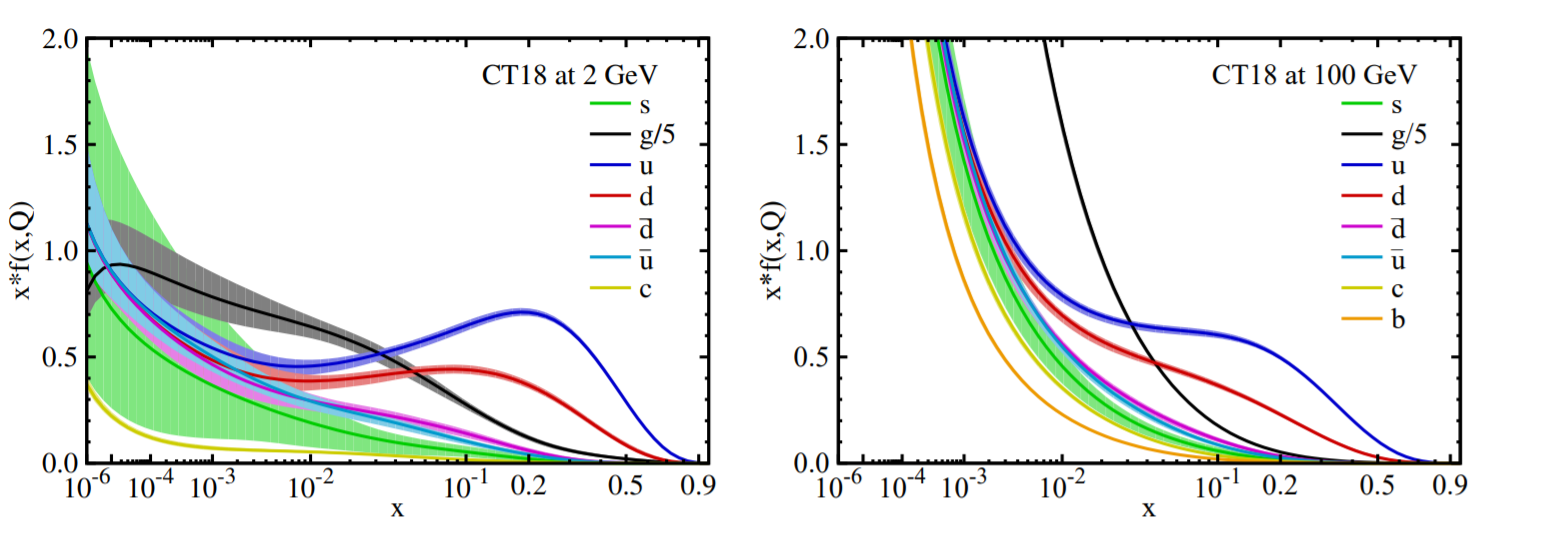
\includegraphics[width=\linewidth]{CT18_PDF.png}
	\caption{\label{fig:PDFs}
		CTEQ-TEA kolektyvo pateikiamos protono partonų pasiskirstymo funkcijos esant skirtingoms susidūrimų energijoms \cite{CTEQ2019}.
		Kairėje -- $Q=2 \; \mathrm{GeV}$, dešinėje -- $Q=100 \; \mathrm{GeV}$.
		Ant horizontalios ašies vaizduojama protono impulso dalis $x$, o ant vertikalios -- tikimybės tankio $f(x,\, Q^2)$
		ir $x$ sandauga.}
\end{figure}

Kvantinės chromodinamikos teorija nenumato partonų pasiskirstymo funkcijų parametrų.
Jie gaunami funkcijas pritaikant prie eksperimentinių tyrimų rezultatų \cite{NNPDF, PDF_ABMP16, CTEQ2019}.
Vieni svarbiausių rezultatų, naudojamų partonų pasiskirstymo funkcijų parametrų nustatymui atkeliauja iš elektrono-protono
sklaidos eksperimentų (anksčiau tokius susidūrimus vykdydavo HERA dalelių greitintuvas Hamburge) bei iš
Drell-Yan proceso, viršūninių kvarkų poros sukūrimo bei vienos čiurkšlės įvykių, kurie vyksta protonų priešpriešinių susidūrimų
metu, tyrimų \cite{CTEQ2019}.
%Turint noro išplėsti dalį apie tyrimus


\subsection{Drell-Yan procesas}
Protonams susiduriant su didžiule energija kvarkas iš vieno protono ir antikvarkas iš kito gali anihiliuoti ir sukurti leptono-antileptono
porą -- elektroną, miuoną arba taoną su atitinkama savo antidalele.
Toks procesas vadinamas Drell-Yan procesu, jis vyksta apsikeičiant $Z$ bozonu arba virtualiu fotonu per s-kanalą:

\begin{equation*}
	q\bar{q} \rightarrow Z/ \gamma^{*} \rightarrow l^{+}l^{-} \; ,
\end{equation*}
čia $q$ ir $\bar{q}$ žymi atitinkamai kvarką ir antikvarką, $\gamma^*$ žymi virtualų fotoną, o $l^+$ ir $l^-$ -- atitinkamai
antileptoną ir leptoną.
Šią reakciją toliau žymėsime $\DY \! \rightarrow \! l^{+}l^{-}$.
Skirtingos Drell-Yan proceso galutinės būsenos, priklausomai nuo to, kokios rūšies leptonai susidaro, yra
vadinamos kanalais: elektronų kanalas, miuonų kanalas, taonų kanalas.
Kadangi taonai gyvuoja labai trumpai, jų kanalo tyrimas yra sudėtingesnis ir dažniausiai yra vykdomas atskirai,
o tuo tarpu elektronų ir miuonų kanalo tyrimus neretai vykdo ta pati mokslinė grupė.

Drell-Yan procesas teoriškai pirmą kartą buvo aprašytas $1970$-aisiais metais.
Tai padarė mokslininkai S.~D.~Drell ir T.~M.~Yan, kurie pritaikė tuo metu dar naują buvusį partonų modelį aprašyti
leptonų poros susidarymui hadronų susidūrimo metu \cite{DYoriginal}.
Drell-Yan procesas pirmą kartą eksperimentiškai buvo stebėtas dar tais pačiais metais protonų susidūrimuose
su urano branduoliais \cite{DY_firstExp}.
Šio proceso tyrimas svarbus todėl, kad jame dalyvauja nevalentinis protono antikvarkas.

Šiais laikais teoretikai Drell-Yan procesą gali sėkmingai aprašyti iki antros eilės (angl.\ \textit{next-to-leading order} -- NLO --
reiškia vienos kilpų ir vienos dalelės išspinduliavimo pataisas) elektrosilpnosios sąveikos
ir trečios eilės kvantinės chromodinamikos perturbacijų tikslumo (angl.\ \textit{next-to-next-to-leading order} -- NNLO --
reiškia dviejų kilpų ir dviejų dalelių išspinduliavimo pataisas).
Tokios aukštos eilės elektrosilpnosios pataisos nenaudojamos, nes kiekvienos elektrosilpnosios viršūnės
indėlis į reakcijos skerspjūvį yra $\approx10$ kartų mažiau reikšmingas (dėl atitinkamai mažesnės sąveikos konstantos), lyginant su
stipriosios sąveikos viršūne.
Drell-Yan proceso pirmos eilės (angl.\ \textit{leading order} -- LO -- reiškia medžio lygmenį) Feinmano diagramos
yra pavaizduotos \ref{fig:DYfeyn}~pav.

\begin{figure}[t]
\centering
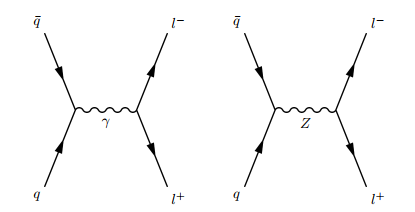
\includegraphics[scale=0.75]{DYprocess.PNG}
\caption{Drell-Yan procesą apibūdinančios medžio lygmens Feinmano diagramos.}
\label{fig:DYfeyn}
\end{figure}

Drell-Yan proceso diferencialinis reakcijos skerspjūvis yra šešiamatis:
$\mathrm{d}^6\sigma/(\mathrm{d}^4p\mathrm{d}\theta^*\mathrm{d}\phi^*$), čia $\sigma$ -- reakcijos skerspjūvis,
$p$ -- leptonų poros keturmatis impulsas (lygus tarpinės dalelės -- $Z$ bozono arba virtualaus fotono keturmačiam
impulsui), $\theta^*$ ir $\phi^*$ -- atitinkamai kampas tarp atlekiančio kvarko (antikvarko) ir išlekiančio leptono (antileptono)
bei azimutinis kampas Collins-Soper atskaitos sistemoje (virtualaus bozono rimties sistemoje) \cite{DYangular}.
Didelių energijų fizikoje keturmatis impulsas dažnai išreiškiamas kaip masės $m=\sqrt{E^2-|\vec{p}|^2}$ (čia $E$ -- energija,
$\vec{p}$ -- trimatis impulso vektorius), skersinio impulso $\pT=\sqrt{p_x^2+p_y^2}$ (čia $p_x$, $p_y$ -- impulso dedamosios
išilgai statmenų protonų susidūrimo krypčiai ašių), spartos $y=\frac{1}{2}\mathrm{ln}[\frac{E+p_z}{E-p_z}]$ (čia $p_z$ -- impulso dedamoji
išilgai lygiagrečios protonų susidūrimo krypčiai ašies) ir
azimutinio kampo $\phi$ rinkinys.
Taigi keturmačio impulso diferencialas $\mathrm{d}^4p$ gali būti pakeistas į $\mathrm{d}m\mathrm{d}\pT\mathrm{d}y\mathrm{d}\phi$.
Be to, šie dydžiai apie procesą gali suteikti gerokai naudingesnės informacijos.

Norint pakankamai tiksliai išmatuoti diferencialinio reakcijos skerspjūvio priklausomybę nuo visų šešių parametrų,
reikėtų labai didelio kiekio duomenų, o taip pat ne visos funkcinės priklausomybės yra vienodai svarbios (pavyzdžiui,
priklausomybė nuo azimutinio kampo $\phi$ yra konstanta, todėl tirti šią priklausomybę nėra prasmės).
Todėl dažniausiai matuojami vienmačiai, dvimačiai arba trimačiai Drell-Yan proceso reakcijos skerspjūviai
\cite{DY_CMS2011, DY_CMS2013, DY_ATLAS2013, DY_ATLAS2014, DY_CMS2015, DY_ATLAS2016, DY_ATLAS2017, DY_CMS2019}.
Nuo skirtingų parametrų priklausančių diferencialinių reakcijos skerspjūvių matavimo rezultatai teoretikams teikia
skirtingą informaciją.

Iš energijos ir impulso tvermės kiekvienoje Feinmano diagramos viršūnėje seka, kad idealiai priešpriešinio susidūrimo metu
Drell-Yan proceso metu sukurtos leptonų poros invariantinė masė (lygi tarpinio bozono masei) medžio lygmenyje priklauso vien
tik nuo susiduriančių protonų impulsų dalių, kurias neša sąveikaujantys partonai:
\begin{align}
\label{eq:DY4vec}
	\begin{bmatrix}
		x_1p_{z\,1} \\		
		0 \\
		0 \\
		x_1p_{z\,1} \\
	\end{bmatrix}
	+
	\begin{bmatrix}
		x_2p_{z\,2} \\
		0 \\
		0 \\
		-x_2p_{z\,2} \\
	\end{bmatrix}
	=
	\begin{bmatrix}
		E_{(\gamma^*\!/\!Z)} \\
		0 \\
		0 \\
		p_{z\,(\gamma^*\!/\!Z)} \\
	\end{bmatrix}
	=
	\begin{bmatrix}
		E_{l1} \\
		p_{x} \\
		p_{y} \\
		p_{z\,l1} \\
	\end{bmatrix}
	+
	\begin{bmatrix}
		E_{l2} \\
		-p_{x} \\
		-p_{y} \\
		p_{z\,l2} \\
	\end{bmatrix}	
	,
\end{align}
iš čia seka, kad
\begin{equation}
\label{eq:DYinvm}
	m^2_{ll} = (E_{l1}+E_{l2})^2-(p_{z\,l1}+p_{z\,l1})^2 = m^2_{(\gamma^*\!/\!Z)} = E^2_{(\gamma^*\!/\!Z)}-p^2_{z\,(\gamma^*\!/\!Z)} =
	(x_1p_{z\,1}+x_2p_{z\,2})^2-(x_1p_{z\,1}-x_2p_{z\,2})^2 ,
\end{equation}
čia $p_{z\,1}$ ir $p_{z\,2}$ -- susiduriančių protonų impulsai, $x_1$ ir $x_2$ -- sąveikaujančių partonų nešamos tų protonų impulsų dalys,
(čia laikome, kad kvarko masė lygi nuliui, todėl jo energija apytiksliai lygi impulso moduliui, o minusu pažymime, kad protonai atlekia
iš priešingų pusių), $E_{(\gamma^*\!/\!Z)}$ ir $p_{z\,(\gamma^*\!/\!Z)}$ -- atitinkamai $Z$ bozono arba virtualaus fotono energija ir
impulsas, $E_{l1}$, $p_{z\,l1}$, $E_{l2}$ ir $p_{z\,l2}$ -- susidariusių leptonų energijos ir impulso $z$ dedamosios, $p_{x}$ ir $p_{y}$ --
leptonų impulsų $x$ ir $y$ dedamosios, kurios dėl impulso tvermės abiems leptonams yra vienodos, bet nukreiptos į priešingas puses.
Čia visur naudojame vienetų sistemą, kurioje $c=1$.
Dėl iš \eqref{eq:DY4vec} ir \eqref{eq:DYinvm} išraiškų sekančios tiesioginės sąsajos tarp matuojamos invariantinės masės ir kvarkų
nešamos protono impulso dalies, diferencialinio reakcijos skerspjūvio $\mathrm{d}\sigma/\mathrm{d}m_{ll}$
matavimai leidžia įvertinti skirtingų partonų su tam tikra protono impulso dalimi egzistavimo tikėtinumus,
t.y., tikslinti partonų pasiskirstymo funkcijas.

Nuo partonų nešamos protono impulso dalies priklauso ir susidariusios leptonų poros sparta.
Partonų nešamas impulso dalis $x_1$ ir $x_2$ per spartą galime išreikšti taip \cite{DYrapi}:
\begin{equation}
	x_{1,2} = \frac{m_{(\gamma^*\!/\!Z)}}{E_1+E_2}e^{\pm y_{(\gamma^*\!/\!Z)}} \, ,
\end{equation}
čia $E_1\!+\!E_2$ -- protonų susidūrimo energija masių centro sistemoje, $y_{(\gamma^*\!/\!Z)}\!=\!y_{ll}$ -- leptonų poros sparta.
Akivaizdu, kad diferencialinio reakcijos skerspjūvio $\mathrm{d}\sigma/\mathrm{d}y_{ll}$ matavimai taip pat gali būti
panaudoti partonų pasiskirstymo funkcijų tikslinimui.
Tuo tarpu diferencialinio reakcijos skerspjūvio $\mathrm{d}\sigma/\mathrm{d}\pT$ matavimai leidžia testuoti aukštesnių eilių
perturbatyvias pataisas.
Iš \eqref{eq:DY4vec} išraiškos seka, kad, Drell-Yan procesą aprašant medžio lygmens diagrama, susiduriančių partonų
(o tai pat ir išlekiančių leptonų) sistemos masės centras turėtų neturėti skersinio judėjimo.
Vis dėlto, skersinis judėjimas atsiranda, kai įskaitome aukštesnių eilių pataisas -- išspinduliavęs gliuoną vienas iš susiduriančių
kvarkų dėl atatrankos gali atšokti ir įgyti judėjimą, statmeną protonų susidūrimo krypčiai.

Diferencialinio reakcijos skerspjūvio $\mathrm{d}\sigma/\mathrm{d}\!\cos\theta^*$ matavimai leidžia tyrinėti Drell-Yan proceso
priekinį-atbulinį asimetriškumą (angl.\ \textit{forward-backward asymmetry}).
Įvykiai su $\cos\theta^*\!\!>\!0$ vadinami priekiniais (angl.\ \textit{forward}), o su $\cos\theta^*\!\!<\!0$ -- atbuliniais
(angl.\ \textit{backward}).
Priekinis-atbulinis asimetriškumas išreiškiamas kaip $A_{FB}=\frac{\sigma_F-\sigma_B}{\sigma_F+\sigma_B}$
(čia $\sigma_F \!=\! \int_0^1\!\frac{\mathrm{d}\sigma}{\mathrm{d\!\cos}\theta^*}\mathrm{d}\!\cos\!\theta^*$ -- priekinio įvykio reakcijos
skerspjūvis, $\sigma_B \!=\! \int_{-1}^0\!\frac{\mathrm{d}\sigma}{\mathrm{d\!\cos}\theta^*}\mathrm{d}\!\cos\!\theta^*$ -- atbulinio įvykio
reakcijos skerspjūvis).
Priekinis-atbulinis asimetriškumas yra tampriai susijęs su svarbiu standartinio modelio parametru -- silpnosios sąveikos maišymosi kampu
(angl.\ \textit{weak mixing angle}) \cite{DYAFB_CMS2011, DYAFB_ATLAS2015, DYAFB_LHCb2015, DYAFB_CMS2018}.
Taigi, Drell-Yan proceso kampinių pasiskirstymų matavimai turi nemažą svarbą šį parametrą nustatant.

Drell-Yan proceso tyrimas taip pat svarbus dėl to, kad jis trukdo tirti kitus standartinio modelio ar hipotetinius procesus, kuriuose
pagaminami du leptonai.
Pavyzdžiui, dviejų leptonų galutinės būsenos nagrinėjamos Higso bozono tyrime \cite{Higgs2018}, ne standartinio modelio dalelės --
$Z'$ bozono -- paieškoje \cite{Zprime}, supersimetrijos paieškoje \cite{SUSYtau} ir pan.
Sėkmingam šių procesų tyrimui svarbu tiksliai įvertinti, kokia išmatuotų pasiskirstymų dalis yra susijusi su Drell-Yan procesu, o
kokia -- su tiriamaisiais procesais.
Didelio tikslumo Drell-Yan proceso tyrimai padeda sumažinti tokių įvertinimų neapibrėžtumus.
Taigi, Drell-Yan proceso matavimai teikia įvairiapusišką naudą teoriniam ir eksperimentiniam dalelių fizikos mokslui.
Toliau šiame darbe bus kalbama apie Drell-Yan proceso diferencialinio reakcijos skerspjūvio $\mathrm{d}\sigma/\mathrm{d}m_{ll}$ matavimą
elektronų ir miuonų kanaluose.

\subsection{Didysis hadronų greitintuvas ir Kompaktiškasis miuonų solenoidas}
Europos branduolinių mokslinių tyrimų organizacijai CERN priklausantis Didysis hadronų priešpriešinių srautų
greitintuvas (angl.\ \textit{Large Hadron Collider} -- LHC) \cite{LHC} yra didžiausias ir galingiausias dalelių greitintuvas pasaulyje.
Tai yra prie Šveicarijos-Prancūzijos sienos įsikūręs, $\sim\!\!100$~m gylyje po žeme esantis žiedinis greitintuvas.
Jo perimetras siekia $27$~km.
Greitintuve galima vykdyti įvairių elektringų hadroninių dalelių (pavyzdžiui, švino branduolių) susidūrimus, tačiau dažniausiai jame
tiriami protonų susidūrimai.
Nuo $2015$ metų Didžiajame hadronų greitintuve vykdomi $13$~TeV energijos protonų susidūrimai.
Dalelės, prieš patekdamos į šį greitintuvą, praeina kelias greitinimo pakopas mažesniuose greitintuvuose, kurie anksčiau buvo
naudojami vykdyti dalelių susidūrimams.
Greitintuve vienu metu gali skrieti iki $2808$ protonų pluoštelių, kurių kiekviename yra apie $10^{11}$ protonų.
Susidūrimai Didžiajame hardonų greitintuve vyksta kas $25$~ns keturiuose žiedo taškuose, aplink kuriuos yra išdėstyti dalelių
detektoriai, priklausantys skirtingų eksperimentų grupėms.
Per vieną protonų pluoštelių prasikeitimą susiduria keliasdešimt protonų porų.
Pluošteliai prakeičiami labai mažu ($\sim\!\!200$~µrad) kampu.
Keturi didžiausi aplink greitintuvą išsidėstę eksperimentai yra CMS, ATLAS, LHCb ir ALICE.
Šiame darbe naudojami 2016 metais CMS eksperimento užregistruoti protonų susidūrimų duomenys.

Kompaktiškasis miuonų solenoidas (angl.\ \textit{Compact Muon Solenoid} -- CMS) \cite{CMSexperiment}
yra plačios paskirties detektorius, galintis detektuoti didelį skaičių skirtingų dalelių.
Jis naudojamas tiek standartinio modelio testavimui ir tikslinimui, tiek naujos fizikos paieškoms.
CMS yra cilindrinės geometrijos, jo aukštis ir plotis -- apytiksliai po $15$~m, o ilgis --
apie $21$~m.
Detektoriaus masė siekia $14000$ tonų, jis susideda iš daug sluoksnių ir segmentų, kurie skirti
skirtingų rūšių dalelėms aptikti.

CMS detektoriaus sluoksnius galima pamatyti \ref{fig:CMSslice} paveiksle.
Kiekvienas subdetektorius turi vieną cilindrinę ir dvi antgalių dalis.
Subdetektorių sluoksniai yra išdėstyti atsižvelgiant į detektuojamų dalelių skvarbumą, kiekvienas sluosknis
yra skirtingas ir turi specifinę paskirtį.

Arčiausiai protonų susidūrimo vietos yra išdėstytas trekų detektorius (angl.\ \textit{silicon tracker}),
pagamintas iš silicio pikselių ir juostelių.
Į nuskurdintą puslaidininkio sluoksnį pataikiusios elektringos dalelės išlaisvina krūvininkus taip sugeneruodamos
elektrinį signalą.
Trekų detektorius turi daug plonų puslaidininkio sluoksnių, tad išanalizavus užregistruotą signalą skirtinguose
sluoksniuose galima nustatyti, kokia kryptimi nulėkė protonų susidūrimo metu sukurtos elektringosios dalelės.
Puslaidininkio sluoksniai padaryti kaip įmanoma plonesni, kad pralėkdama dalelė juose prarastų kuo mažiau energijos
ir nepakeistų savo trajektorijos.

Pralėkusios trekų detektorių dalelės pirmiausia pataiko į elektromagnetinį kalorimetrą (angl.\ \textit{Electromagnetic Calorimeter} -- ECAL).
Šio subdetektoriaus paskirtis -- detektuoti elektronus ir fotonus bei išmatuoti jų energiją.
Elektromagnetinis kalorimetras pagamintas iš scintiliuojančios medžiagos -- švino volframato $\mathrm{PbWO}_{4}$.
Į elektromagnetinį kalorimetrą pataikius reliatyvistiniu greičiu lekiančiam elektronui, medžiagos elektronai yra sužadinami
ir relaksuoja skleisdami šviesą.
Elektrono energija nustatoma išmatavus švytėjimo intensyvumą, kuris yra proporcingas elektrono prarastai energijai medžiagoje.
Elektronas kalorimetre yra visiškai sustabdomas.
Į tankią scintiliatoriaus medžiagą pataikę fotonai pavirsta į elektrono-pozitrono porą, kurios energija jau gali būti išmatuojama
tokiu pačiu būdu.
Ar signalas elektromagnetiniame kalorimetre yra susijęs su elektronu, ar su fotonu galima atskirti pagal tai, ar jis yra susietas su
trekų detektoriuje užregistruotu treku.

Dalelės, kurios nėra sustabdomos elektromagnetiniame kalorimetre, pataiko į hadronų kalorimetrą (angl.\ \textit{hadron calorimeter} -- HCAL).
Šis subdetektorius sustabdo hadronus ir matuoja jų energiją.
Hadronų kalorimetre naudojamas plastiko scintiliatorius.
Kadangi hadronai yra gerokai sunkesni ir skvarbesni už elektronus, norint juos sustabdyti tarp scintiliatoriaus sluoksnių yra įterptos
vario plokštės, o taip pat šis subdetektorius yra gerokai storesnis už elektromagnetinį kalorimetrą.

Už hadronų kalorimetro yra iki superlaidumo temperatūros atšaldytas solenoidinis elektromagnetas.
Kai detektorius yra įjungtas, solenoidu teka maždaug $19.1$~kA stiprio elektros srovė, sukurianti iki $4$~T siekiantį magnetinį lauką.
Jo paskirtis -- iškreivinti krūvį turinčių dalelių trajektorijas.
Pagal tai, kuria kryptimi dalelės trajektorija užsisuka, galima nustatyti dalelės elektrinį krūvį,
o iš trajektorijos kreivumo spindulio galima įvertinti ir jos skersinį impulsą.
Taip pat solenoidas veikia kaip papildoma kliūtis skvarbiausiems hadronams.
Vis dėlto, norint užtikrinti, kad kuo mažiau hadronų pasiektų tolimesnius detektoriaus sluoksnius, už
solenoido yra sumontuotas papildomas hadronų kalorimetro sluoksnis, vadinamas išoriniu hadronų kalorimetru
(angl.\ \textit{HCAL outer}).

Pačioje CMS detektoriaus išorėje keliais sluoksniais išdėstyti miuonų detektoriai.
Miuonai yra apie $200$ kartų sunkesni už elektronus, bei nesąveikauja stipriąja sąveika, todėl yra gerokai skvarbesni
už visas kitas detektuojamas daleles.
Dėl šios priežasties jie nėra sustabdomi nei elektromagnetiniame, nei hadronų kalorimetruose.
Miuonų detektoriai veikia dujų išlydžio principu -- bet kokia detektoriaus išorę pasiekusi elektringa dalelė jonizuoja
miuonų detektoriuose esančias dujas.
Per jonizuotas dujas pratekėjusi elektros srovė užfiksuojama kaip pataikymas.
Nors miuonų detektoriai galėtų registruoti bet kokių elektringų dalelių pataikymus, dažniausiai visos
kitos dalelės yra sustabdomos ankstesniuose detektoriaus sluoksniuose.
Tuo tarpu miuonai nėra sustabdomi net ir miuonų detektorių sistemoje -- dujiniai detektoriai tik užfiksuoja jų
trajektoriją.
Šių dalelių impulsas yra nustatomas iš jų trajektorijos kreivumo.
Kad impulsą būtų galima nustatyti kuo efektyviau, tarp miuonų detektorių yra sumontuotos geležinės magnetinio
lauko apgrąžos plokštės, kurios sustiprina magnetinį lauką miuonų detektoriuose, tuo pačiu neleisdamos jam tęstis toli
už detektoriaus ribų.
Taip pat šios plokštės užblokuoja kelią paskutinėms iki jų prasiskverbusioms dalelėms, kurios nėra miuonai
arba neutrinai.
Neutrinai yra vienintelės dalelės, kurios CMS detektoriumi nedetektuojamos.
Vis dėlto, neutrino pėdsaką galima nuspėti apskaičiavus visų užregistruotų dalelių skersinių impulsų vektorinę sumą
(susiduriantys protonai juda išilgai $z$ ašies, todėl visų susidariusių dalelių skersinių impulsų vektorinė suma turėtų
būti lygi nuliui) ir pastebėjus didelį skersinio impulso trūkumą tam tikra kryptimi.

\begin{figure}[t]
	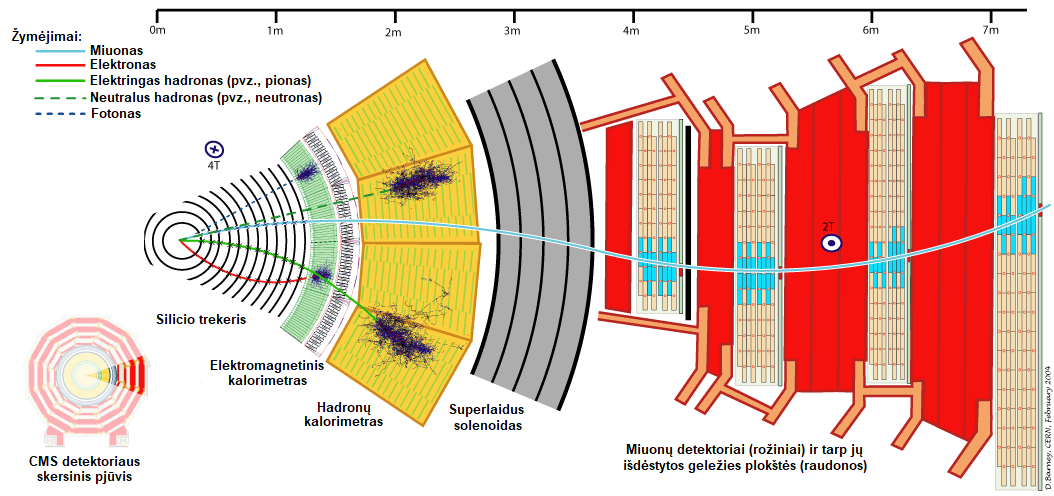
\includegraphics[width=\textwidth]{CMSslice_LT.png}
	\caption{\label{fig:CMSslice}Skersinis CMS detektoriaus pjūvis \cite{CMSslice}.
	Skirtingos linijos žymi įvairių dalelių, išlekiančių iš protonų susidūrimo vietos, trajektorijas.
	Trūki linija žymi elektriškai neutralios dalelės trajektoriją, kuri silicio trekų detektoriuje
	neužfiksuojama.}
\end{figure}

\subsection{Trigeriai}
Per kiekvieną protonų pluoštelių pasikeitimo įvykį (toliau juos vadinsime tiesiog įvykiais) CMS detektorius
užregistruoja apie $1$ MB informacijos \cite{CMScomputing}.
Norint išsaugoti kiekvieną kas $25$~ns vykstantį įvykį reikėtų ypatingai greitos elektronikos, gebančios išrašyti
duomenis $\sim\!\!40$~TB/s greičiu, o taip pat ir nerealiai didelių duomenų saugyklų.
Vis dėlto, labai didelė šių įvykių dalis mokslininkams nėra įdomi -- tai nepakankamai energingi susidūrimai
arba labai dažnai vykstantys ir jau gerai ištirti procesai.
CMS eksperimente išsaugomų įvykių skaičiui sumažinti (stengiantis atmesti kiek įmanoma daugiau neįdomių ir palikti
kuo daugiau įdomų įvykių) naudojama dviejų lygių trigerių sistema, susidedanti iš pirmo lygio
(angl.\ \textit{level} 1 -- L1) ir aukšto lygio (angl.\ \textit{high-level trigger} -- HLT) trigerių \cite{CMStrig}.

Pirmojo lygio trigeris -- tai šalia detektoriaus sumontuota specialiai tam sukurta kompiuterinės įrangos sistema.
Ši sistema realiu laiku minimaliai apdoroja kalorimetrų bei miuonų detektorių duomenis ir atrenka įvykius, atsižvelgiant
į juose esančius fizikinių objektų kandidatus (signalas miuonų detektoriuose gali reikšti miuoną, signalai kalorimetruose --
elektroną, fotoną, hadronus, signalo kalorimetruose trūkumas -- neutrinus).
Galutinis pirmo lygio trigerio atrankos etapas -- papildomų kriterijų, kurie gali būti pasirinkti iš programuojamo
kriterijų meniu, pritaikymas.
Šie papildomi kriterijai gali būti keičiami ir greitintuvui veikiant, priklausomai nuo jo veikimo sąlygų
(su greitintuvu dirbantys mokslininkai kartais eksperimentuoja keisdami protonų skaičių per vieną protonų prasikeitimą).
Kriterijus visada stengiamasi parinkti taip, kad juos praeitų ne daugiau kaip $10^5$ įvykių per sekundę
(tai yra CMS elektronikos pajėgumų viršutinė riba).
Jie gali būti tokie, kaip reikalavimas fizikinio objekto kandidatui viršyti tam tikrą slenkstinę energiją, reikalavimas
viename įvykyje būti tam tikram skaičiui objekto kandidatų ir pan.
Pirmo lygio trigeris turi apytiksliai $4$~µs vėlavimą, per kurį sistema nusprendžia, ar įvykis turėtų būti
išsaugomas tolimesnei analizei. 

Aukšto lygio trigeris -- tai programinės įrangos rinkinys, skirtas detaliau išanalizuoti pirmo lygio trigerį praėjusius
įvykius ir dar labiau sumažinti jų skaičių prieš išrašant juos ilgalaikiam saugojimui.
Aukšto lygio trigerio programinė įranga yra sudiegta į įprastus superkompiuterius, pastatytus netoli CMS detektoriaus.
Juose įvykio vaizdas atkuriamas pasinaudojant pilna detektoriaus užregistruota informacija, o atpažintiems fizikiniams
objektams, siekiant išsaugoti tik potencialiai įdomius įvykius, pritaikomi griežtesni atrankos kriterijai.
Aukšto lygio trigeris sumažinta išsaugomų duomenų kiekį iki maždaug $400$ įvykių per sekundę.
Šie įvykiai yra įrašomi ilgalaikiam saugojimui, kad vėliau galėtų būti analizuojami mokslininkų.

Neretai Didžiajame hadronų greitintuve protonų susidūrimų skaičius per vieną pluoštelių prasikeitimą pakeliamas iki tiek,
kad net ir potencialiai įdomūs įvykiai įvyksta taip dažnai, kad jų visų tampa nebeįmanoma išsaugoti.
Tokiu atveju, tiek pirmo, tiek aukšto lygio trigeriuose gali būti panaudojamas nustatyto dydžio tarpavimas (angl.\ \textit{prescale}),
kuris atmeta fiksuotą porciją potencialiai įdomių įvykių.
Pavyzdžiui, dvejetui lygus tarpavimas sumažins išsaugomų potencialiai įdomių įvykių skaičių perpus.


\subsection{Protonų susidūrimo įvykių atkūrimas}
CMS detektoriaus užregistruoti signalai sujungiami į pilną protonų susidūrimo įvykio vaizdą naudojantis
dalelių srauto (angl.\ \textit{Particle Flow} -- PF) algoritmu \cite{ParticleFlow}.
Šis algoritmas sujungia trekų detektoriuje užregistruotus signalus su pataikymais į kalorimetrus arba miuonų
detektorius, taip nustatydamas susidariusių dalelių tipus, jų trajektorijas bei kitus parametrus
(energiją, impulsą, elektrinį krūvį ir pan.).
Dalelių srautas gali atkurti ne tik dalelių trajektorijas, bet ir kitus fizikinius objektus, pavyzdžiui,
hadronų čiurkšles (ši sąvoka plačiau paaiškinta \ref{sec:jets} skyriuje) ar skersinio impulso trūkumą.

Dalelių srauto algoritmas įvykių atkuria iteratyviai.
Pirmiausia nustatomos \ltq{akivaizdžiausios} trajektorijos (pavyzdžiui, tokios, kurios susideda iš pataikymų
kiekviename trekų detektoriaus sluoksnyje, gerai sutampa su pataikymais į kalorimetrus ar miuonų detektorius,
kalorimetro išmatuota energija gerai tinka su impulsu, nustatytu iš trajektorijos kreivumo ir pan.).
Tada signalai, kurie buvo panaudoti nustatant geriausias trajektorijas, pašalinami ir atkūrimo procedūra
kartojama su tuo, kas liko, tik šiek tiek sušvelninus trajektorijos nustatymo \ltq{gerumo} reikalavimus.
Taip iteruojama iki kol panaudojama visa detektoriaus užregistruota informacija.
Galų gale gaunamas platus galutinių įvykio produktų sąrašas, leidžiantis pamatyti pilną protonų susidūrimo įvykio vaizdą,
kurį jau gali analizuoti mokslinės tyrimų grupės.
Atkurto Drell-Yan proceso įvykio kandidato pavyzdys atvaizduotas \ref{fig:Event} paveiksle.
Įvykio vaizdas sugeneruotas naudojantis CMS programinės įrangos pakete esančia programa FireWorks.

Per kiekvieną protonų pluoštelių prasikeitimą įvyksta kelios dešimtys protonų susidūrimų, o taip pat, iki kol
visos susidariusios dalelės išlekia iš detektoriaus arba yra sustabdomos, jau būna prasidėjęs kitas pluoštelių
prasikeitimas (daugybiniai protonų susidūrimai angliškai vadinami \textit{pile-up} -- PU).
Iš kelių dešimčių vienu metu įvykusių protonų susidūrimų dažniausiai įdomus būna tik vienas (o įvykiuose, kurių
nepraleido trigeris, įdomaus nebuvo nei vieno).
Dalelių srauto algoritmas sugeba atskirti didžiąją dalį dalelių trajektorijų, susijusių su pašaliniais
protonų susidūrimais ir jas atmesti.
Iš tiesų, dalelių srauto algoritmas yra toks pajėgus, kad net geba atpažinti daleles, kurios atsirado kitų dalelių skilimo metu
ar susieti užregistruotus fotonus su juos dėl judėjimo su pagreičiu magnetiniame lauke išspinduliavusiais elektronais.
Norint sėkmingai taikyti tokį algoritmą svarbu, kad aktyvių detektoriaus elementų sudalinimas būtų kuo smulkesnis,
o pats detektorius būtų sandarus.
CMS detektorius gerai atitinka abu iš šių kriterijų.

\begin{figure}[t]
	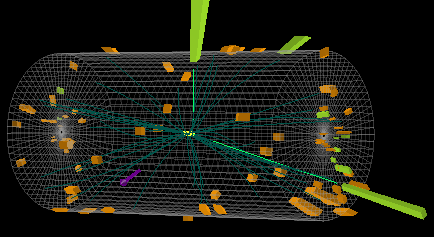
\includegraphics[width=0.8\textwidth]{Event.png}
	\caption{\label{fig:Event}
		Dalelių srauto algoritmu atkurto Drell-Yan proceso įvykio kandidato vaizdas.
		Tamsiai žalios linijos vaizduoja mažos energijos dalelių (daugiausia pionų) trajektorijas,
		o ryškios šviesiai žalios -- didelės energijos elektronų trajektorijas.
		Šviesiai žali ir oranžiniai stulpeliai vaizduoja atitinkamai elektromagnetinio ir hadronų kalorimetro
		segmentuose užregistruotus energijos kiekius.
		Atkurtame įvykyje matomos elektronų poros invariantinė masė apytiksliai lygi $90$ GeV, t.y., labai artima $Z$ bozono masei.
	}
\end{figure}


\subsection{Signalas ir triukšmas}\label{sec:sig_bkg}
Drell-Yan proceso metu susidaro du priešingo elektrinio krūvio izoliuoti (neapsupti pašalinių dalelių) leptonai.
Izoliuotų leptonų pora gali susidaryti ir kitų procesų metu.
Atskirai paėmus kiekvieną detektoriaus užregistruotą įvykį neįmanoma vienareikšmiškai teigti, kad tai yra Drell-Yan
arba kito proceso įvykis.
Pašaliniai procesai, kurie dėl savo galutinių produktų panašumo trukdo tirti Drell-Yan procesą, vadinami triukšmo įvykiais.
Tuo tarpu Drell-Yan proceso įvykiai vadinami signalu.
Didžiajame hadronų greitintuve vykdomiems Drell-Yan proceso matavimams pagrindiniai triukšmai, susiję su izoliuotais
leptonais (proceso tikėtinumo didėjimo tvarka) yra šie:
\begin{itemize}
	\item Vieno viršūninio kvarko ir $W$ bozono įvykiai ($tW$ arba $\tbarW$), kai tiek $W$ bozonas, tiek viršūninis kvarkas
	skyla leptoniškai
	\item Dviejų masyvių leptoniškai skylančių vektorinių bozonų įvykiai ($WW$, $\WZ$ ir $\ZZ$)	
	\item Viršūninio kvarko ir antikvarko poros ($\ttbar\,$) įvykiai, kai abu viršūniniai kvarkai skyla leptoniškai
	\item Drell-Yan proceso taonų kanalas ($\DYtau$), kai taonai skyla į lengvesnius leptonus
\end{itemize}
Yra žinoma, kad su $WW$, $\WZ$, $\ZZ$, $tW$, $\tbarW$ ir $\ttbar$ procesais susiję triukšmai yra svarbūs visoje invariantinės
masės srityje, tuo tarpu $\DYtau$ -- žemos invariantinės masės (maždaug $40-80$~GeV) srityje
\cite{DY_CMS2011, DY_CMS2013, DY_CMS2015, DY_CMS2019}.
Taip pat galimi triukšmo įvykiai, susiję su dalelių srauto algoritmo neteisingai atpažintais fizikiniais objektais.
Dažniausi tokio tipo triukšmai siejasi su čiurkšlėmis, kurios buvo klaidingai atpažintos kaip izoliuoti leptonai.
Apie šiuos triukšmus plačiau rašoma \ref{sec:jets} skyriuje.

Matuojant Drell-Yan proceso diferencialinį reakcijos skerspjūvį stengiamasi tiriamą fazinę erdvę apriboti taip, kad būtų
atmetama kiek įmanoma daugiau triukšmo įvykių, tuo pačiu išsaugant kuo didesnį signalo įvykių skaičių.
Vis dėlto, net į apribotą tyrimo sritį patenka reikšmingas triukšmo įvykių skaičius.
Šį įvykių skaičių reikia įvertinti kaip įmanoma tiksliau ir jį atmesti iš tiriamų pasiskirstymų.

\subsection{Su čiurkšlėmis susiję triukšmo įvykiai}\label{sec:jets}
Protonų susidūrimuose galutinė įvykio būsena (angl.\ \textit{final state} -- taip vadinamas iš procesą aprašančios
Feinmano diagramos išeinančių dalelių rinkinys -- reakcijos produktas) dažnai yra palydima vieno ar kelių kvarkų ir/arba gliuonų,
(jeigu neskaičiuojame likusių partonų, kurie nesusąveikauja ir nulekia apytiksliai tiesiai).
Pavyzdžiui, energingą kvarką arba gliuoną prieš sąveikaudami gali išspinduliuoti reakcijoje dalyvaujantys partonai.
Įvykio metu sukurtos masyvios dalelės (taonai, $W$, $Z$ ir Higso bozonai) su tam tikra tikimybe taip pat gali skilti į kvarkus.
Vis dėlto, izoliuotų kvarkų arba gliuonų dalelių detektoriais aptikti neįmanoma.

Daug energijos turintys kvarkai ją praranda spinduliuodami gliuonus.
Tuo tarpu gliuonai gali skilti į kvarko ir antikvarko poras arba patys spinduliuoti papildomus gliuonus.
Tokiu būdu iš vieno galutinės būsenos partono pagaminamas \ltq{partonų dušas} (angl.\ \textit{parton shower}).
Kai partonų duše esančių dalelių energija pasidaro pakankamai maža, stipriosios sąveikos konstanta išauga iki
tiek, kad perturbatyvus kvantinės chromodinamikos aprašymas nustoja būti validus.
Prie žemų energijų ($<\!1$~GeV) pasireiškia kvarkų \ltq{įkalinimas} (angl.\ \textit{confinement}): dėl sąveikos stiprumo
kvarkai gali egzistuoti tik grupėse, kuriose jų spalvinis krūvis neutralizuojamas.
Šiame režime bandant kvarkus vieną nuo kito atitraukti reikėtų tiek energijos, kad jos užtektų iš vakuumo pagaminti
naujai kvarko-antikvarko porai, kuri suformuotų naujas grupes su atitrauktais kvarkais ir neutralizuotų jų spalvinį krūvį.
Dėl šio reiškinio partonų duše lekiantys kvarkai ir gliuonai pradeda formuoti hadronus.
Tai vadinama hadronizacija.
Jos metu hadronų pagaminama labai daug, tad vieno energingo partono pėdsaką detektorius užregistruoja kaip besiplečiančio
kūgio formos dalelių srautą, sudarytą iš daugybės įvairių rūšių hadronų bei kitų dalelių \cite{Jets}.
Šie dalelių srautai vadinami čiurkšlėmis (angl.\ \textit{jets}).

Čiurkšlėse dažniausiai susidaro ne tik hadronai.
Pavyzdžiui, čiurkšlėse galimas nemažas skaičius fotonų, kurie atsiranda daugiausia iš neutralaus piono skilimų.
Taip pat vykstant didelės energijos partonų sklaidos procesams galima sukurti sunkiųjų kvarkų, kurie gyvuoja trumpai
ir skildami gali pagaminti leptonų.
Pavyzdžiui, elektronas arba miuonas yra randamas apytiksliai $20\%$ gelminio kvarko sukurtų čiurkšlių
(angl.\ \textit{b-jets}) ir apytiksliai $10\%$ žaviojo kvarko sukurtų čiurkšlių (angl.\ \textit{c-jets}) \cite{LeptonJets}.
Čiurkšlėse susidariusios stipriąja sąveika nesąveikaujančios dalelės neretai pagelbėja nustatant,
kokį kvarką atitinka matoma čiurkšlė \cite{LeptonJets}.
Vis dėlto, jos kartais gali ir suklaidinti -- retais atvejais čiurkšlės yra supainiojamos su protonų susidūrimo metu
pagamintu leptonu
\cite{DY_CMS2011, DY_CMS2013, DY_ATLAS2013, DY_ATLAS2014, DY_CMS2015, DY_ATLAS2016, DY_ATLAS2017, DY_CMS2019, EleID, MuonID}.

Bendru atveju čiurkšlėse susidarę leptonai nėra izoliuoti -- jie yra apsupti hadronų srauto.
Vis dėlto, pasitaiko atvejų, kai leptonas yra pakankamai energingas, kad susumuotas aplink lėkusių hadronų ir fotonų
skersinis impulsas yra gerokai mažesnis už leptono impulsą (tai gali sudaryti įspūdį, kad leptonas yra izoliuotas).
Taip pat galimi atvejai, kai didesnę dalį čiurkšlės energijos nešasi vienas ar keli fotonai.
Įvykio atkūrimo algoritmui klaidingai priskyrus trekų detektoriuje užfiksuotą trajektoriją su fotonų paliktu signalu
elektromagnetiniame kalorimetre čiurkšlę galima neteisingai atpažinti kaip elektroną.
Jeigu tokio \ltq{netikro} elektrono energija išmatuojama gerokai didesnė už jį supančių hadronų energiją, galima ji
klaidingai palaikyti izoliuotu.
Labai retais atvejais nutinka ir taip, kai energinga čiurkšlė pralekia hadronų kalorimetrą ir palieka signalą miuonų
detektoriuje (toks procesas angliškai vadinamas \textit{hadronic punchthrough}).
Jeigu \ltq{netikro} miuono trajektorija dalelių srauto algoritmo yra atkuriama kaip ganėtinai tiesi (o tai reiškia
didelį skersinį impulsą), įmanoma netgi klaidingai pagalvoti, kad jis yra izoliuotas.
Prie klaidingo čiurkšlių atpažinimo gali prisidėti ir neidealus detektoriaus bei trajektorijų atkūrimo efektyvumas
(nebūtinai bus užfiksuotos visos čiurkšlėje susidariusios dalelės).

Pagrindiniai su klaidingai atpažintomis čiurkšlėmis susiję Drell-Yan proceso triukšmo įvykiai yra $W$ bozono ir vienos čiurkšlės
įvykiai ($\WJets$) bei stipriosios sąveikos nulemti kelių čiurkšlių įvykiai (sutrumpintai žymimi $\QCD$).
Yra žinoma, kad miuonų kanale su čiurkšlėmis susiję triukšmai turi reikšmingą indėlį žemos invariantinės masės,
o elektronų kanale -- visoje invariantinės masės srityje \cite{DY_CMS2011, DY_CMS2013, DY_CMS2015, DY_CMS2019}.
Tiriant Drell-Yan procesą, į šių triukšmo procesų indėlį taip pat svarbu atsižvelgti.

\subsection{Triukšmo įvykių skaičiaus įvertinimas}
Turint detektoriaus išmatuotų duomenų rinkinį neįmanoma vienareikšmiškai pasakyti, kurie įvykiai yra susiję su triukšmo
procesais.
Galima tik ribotu tikslumu įvertinti, koks skaičius triukšmo įvykių rinkinyje galėjo būti.
Triukšmo įvykių skaičius įvertinamas pasinaudojant papildomais duomenų rinkiniais, kurie gali būti gauti iš tikro matavimo
arba sumodeliuoti.

Grubų triukšmo įvykių skaičiaus įvertį galima gauti pasinaudojus Monte Carlo (MC) metodu sumodeliuotais protonų susidūrimo įvykiais.
Įvykių modeliavimas būna atliekamas keliais lygmenimis.
Pirmiausia sumodeliuojamas pats protonų susidūrimas ir gaunama, kokios dalelės susidarė jo metu.
Tada modeliuojami po susidūrimo vykstantys antriniai procesai, tokie, kaip hadronizacija, spinduliavimas, dalelių skilimai,
pašaliniai protonų susidūrimai, vykstantys tuo pačiu metu.
Galiausiai modeliuojama, kaip įvykio produktai sąveikauja su medžiaga -- detektoriaus komponentais.
Tokį virtualų eksperimentą kartojant daug kartų galima gauti vidutinį rezultatą, kuris yra palyginamas su realiu eksperimentu.

Vis dėlto, sumodeliuoti įvykius taip, kad virtualaus eksperimento sąlygos idealiai atitiktų realaus eksperimento sąlygas,
yra praktiškai neįmanoma.
Atsižvelgiant į kai kuriuos neatitikimus modeliuotiems įvykiams gali būti pritaikomos CMS eksperimento mokslinių grupių
rekomenduojamos pataisos.
Tačiau vis tiek egzistuoja modeliavimo neapibrėžtumų, kurie kenkia įverčio kokybei (pavyzdžiui, nepakankamos žinios apie
atskirų triukšmo procesų įvykių tikėtinumus, neidealus detektoriaus atsako modeliavimas, papildomi protonų susidūrimai ir pan.).
Blogiausiai modeliavimas įvertina procesus, kurių tikėtinumas labai didelis, o įvykių atrankos praėjimo efektyvumas labai
mažas -- norint gauti tolydų ir tikrovišką pasiskirstymą reikėtų tokių įvykių sumodeliuoti nepaprastai daug, o tam
reikalingi neįmanomai dideli skaičiavimo ir duomenų saugojimo resursai.
Būtent tokie yra su klaidingai atpažintomis čiurkšlėmis susiję W+Jets ir QCD procesai -- jų tikėtinumas didesnis už
Drell-Yan proceso (atitinkamai $3$ ir net $500$ kartų), o tikimybė čiurkšlei būti klaidingai atpažintai kaip analizei
atrinktam leptonui yra ganėtinai maža. 
Dėl šių trūkumų naudoti vien modeliuotus duomenis yra vengiama ir, kur įmanoma, stengiamasi triukšmo įvykių skaičių
įvertinti naudojant matavimu grįstus metodus.

Matavimu grįsti (angl.\ \textit{data-driven}) metodai apjungia matavimą ir modeliavimą, kad būtų gautas kuo
tikroviškesnis įvykių skaičiaus įvertis.
Šių metodų veikimo principas remiasi signalo ir kontrolinės sričių apibrėžimais.
Signalo sritis pasirenkama taip, kad į ją patektų kuo daugiau signalo ir kuo mažiau triukšmo įvykių -- tai yra pagrindinė
tyrimo sritis.
Kontrolinė sritis pasirenkama taip, kad į ją patektų kuo daugiau triukšmo ir kuo mažiau signalo įvykių.
Sritys gali būti apibrėžiamos įvairiais užregistruotus įvykius apibūdinančių parametrų apribojimais, pavyzdžiui,
apribojant tam tikrų įvykyje užregistruotų dalelių ar čiurkšlių skaičių, tiriamų dalelių trajektorijų izoliuotumą, jų
elektrinius krūvius ir pan.
Signalo ir kontrolinė sritys turi būti nepersidengiančios.
Matavimu grįsti metodai nustato sąsają tarp triukšmo įvykių pasiskirstymo signalo ir kontrolinėje srityje.
Tada triukšmo įvykių skaičius, apskaičiuotas kontrolinėje srityje, ekstrapoliuojamas į signalo sritį.
Šiais laikais atliekamuose Drell-Yan proceso diferencialinio reakcijos skerspjūvio matavimuose populiarūs yra šie matavimu
grįsti metodai: $\emu$ metodas \cite{DY_CMS2011, DY_CMS2013, DY_ATLAS2014, DY_CMS2015, DY_CMS2019},
ABCD metodas \cite{DY_CMS2011, DY_CMS2013, DY_ATLAS2014, DY_CMS2015, DY_ATLAS2016, DY_ATLAS2017},
klaidingo atpažinimo metodas \cite{DY_CMS2011, DY_CMS2013, DY_ATLAS2013, DY_CMS2015, DY_ATLAS2016, DY_CMS2019}.
Jei triukšmo įvykyje susidaro dvi nestabilios dalelės, kurios gali skilti į izoliuotus leptonus nepriklausomai
(tokį aprašymą atitinka $tW$, $\tbarW$, $WW$, $\ttbar\,$ ir $\DYtau$ procesai), jo indėlis gali būti įvertintas $\emu$ metodu.
Įvykiams, susijusiems su klaidingai atpažintomis čiurkšlėmis, įvertinti gali būti naudojami klaidingo atpažinimo ir ABCD metodai.
Toliau šiame darbe bus gilinamasi į klaidingo atpažinimo metodą.


\subsection{Klaidingo atpažinimo metodas}
Klaidingo atpažinimo metodas yra ganėtinai populiarus nustatant triukšmo įvykių skaičių, kuriuose viena ar kelios čiurkšlės
buvo klaidingai atpažintos kaip izoliuoti leptonai.
Nemažas skaičius CMS ir ATLAS eksperimentuose vykdomų leptono-antileptono galutinės būsenos tyrimų (daugiausia tai yra
Drell-Yan proceso tyrimai arba naujų didelės masės bozonų paieška) vienaip ar kitaip šį metodą naudoja
\cite{DY_CMS2011, DY_CMS2013, DY_ATLAS2013, DY_CMS2015, DY_ATLAS2016, DY_CMS2019, Z'_ATLAS2011, Z'_CMS2011, Z'_CMS2012,
Z'_CMS2013, Z'_ATLAS2014, Z'_CMS2015, Z'_CMS2017, Z'_CMS2018}.
Vis dėlto, daugelyje viešai prieinamų straipsnių klaidingo atpažinimo teorinis veikimo principas nėra aprašytas, arba tai padaryta
labai minimaliai.
Ypatingai CMS kolektyvo straipsniuose daugiau koncentruojamasi į praktinius klaidingo atpažinimo metodo aspektus.
Nepaisant to, galima susidaryti bendrą įspūdį, kad klaidingo atpažinimo metodo taikymas susideda iš dviejų dalių:
pirmiausia įvertinama klaidingo atpažinimo tikimybė, o tada gauta tikimybės vertė panaudojama kaip svorinis
daugiklis įvykiams, kurie nepraėjo pagrindinės tyrimo atrankos.

Įprastai klaidingo atpažinimo tikimybė yra įvertinama pasinaudojant duomenų rinkiniu, gaunamu smarkiai atlaisvinus
tyrimui naudojamus atrankos kriterijus.
Šis duomenų rinkinys apdorojamas taip, kad jame liktų vien tik klaidingai kaip leptonai atpažintos čiurkšlės.
Tada skaičiuojama, kokia dalis klaidingai atpažintų čiurkšlių patenka į tiriamąją (signalo) sritį
\cite{DY_ATLAS2016, Z'_ATLAS2011, Z'_CMS2011, Z'_ATLAS2014, Z'_CMS2015}.
Gautas santykis yra vadinamas klaidingo atpažinimo tikimybe.
Toliau ją žymėsime raide $f$.
Klaidingo atpažinimo tikimybė dažniausiai matuojama kaip funkcija nuo kelių parametrų.
Įvertinta tikimybė pritaikoma įvertinant, kiek su klaidingai atpažintomis čiurkšlėmis susijusių įvykių
galėjo praeiti dviejų leptonų įvykių atranką.
Tam pasinaudojama įvykių rinkiniais, kuriuose vienas arba abu leptonai nepraėjo signalo atrankos kriterijų.
Dažniausiai klaidingo atpažinimo tikimybė pritaikoma kaip svoris daugiklis šiems įvykiams \cite{Z'_ATLAS2011, Z'_CMS2011, Z'_CMS2015}.
Įvykio svoris susideda iš daugiklio $f/(1-f)$ kiekvienam objektui, kuris nepraėjo signalo atrankos (t.y., visas įvykio svoris
susideda iš vieno arba dviejų tokių daugiklių) \cite{Z'_CMS2015}.
Šie svoriai transformuoja įvykių su atrankos nepraeinančiais leptonais pasiskirstymą į pasiskirstymą, atitinkantį signalo
srityje esančius įvykius.

Kai kurios ATLAS eksperimentinės tyrimo grupės klaidingo atpažinimo tikimybės pritaikymą aprašo kitaip \cite{DY_ATLAS2016, Z'_ATLAS2014}.
Jeigu įvertiname ne tik tikimybę klaidingai atpažintai čiurkšlei patekti į signalo sritį, bet ir tikimybę \ltq{tikram}
elektronui patekti į signalo sritį (angl.\ \textit{acceptance}, toliau šį dydį žymėsime raide $a$), galime gauti lygčių sistemą,
susiejančią įvykius su \ltq{tikrais} arba \ltq{netikrais} leptonais ir detektoriaus registruojamus įvykius su objektais signalo
arba kontrolinėje srityse:

\begin{align}
\label{eq:FRmatrix}
	\begin{bmatrix}
		N_{SS} \\		
		N_{SC} \\
		N_{CS} \\
		N_{CC} \\
	\end{bmatrix}
	=
	\begin{bmatrix}
		a_1a_2 & a_1f_2 & f_1a_2 & f_1f_2 \\
		a_1(1-a_2) & a_1(1-f_2) & f_1(1-a_2) & f_1(1-f_2) \\
		(1-a_1)a_2 & (1-a_1)f_2 & (1-f_1)a_2 & (1-f_1)f_2 \\
		(1-a_1)(1-a_2) & (1-a_1)(1-f_2) & (1-f_1)(1-a_2) & (1-f_1)(1-f_2) \\
	\end{bmatrix}
	=
	\begin{bmatrix}
		N_{RR} \\
		N_{RF} \\
		N_{FR} \\
		N_{FF} \\
	\end{bmatrix}
	\! ,
\end{align}
čia $N$ žymi įvykių skaičių, indeksai $S$ ir $C$ -- atitinkamai leptono objektą, patenkantį į signalo arba kontrolinę sritį,
o indeksai $R$ ir $F$ -- atitinkamai tikrą ir netikrą leptonus.
Detektorius išmatuoja įvykių skaičius $N_{SS}$, $N_{SC}$ ir t.t., o tyrėjus iš tikrųjų dominantys dydžiai $N_{RF}$, $N_{FR}$ ir
$N_{FF}$ (įvykiai su klaidingai atpažintomis čiurkšlėmis) gali būti gauti invertavus \eqref{eq:FRmatrix} išraiškoje esančią matricą.

Taigi, nors klaidingo atpažinimo metodas viešai prieinamoje literatūroje nėra labai išsamiai aprašytas, galima susidaryti įspūdį, jog
jo įgyvendinimas nėra vienareikšmis: jis gali turėti nemažai variacijų ir konkreti metodika turi būti adaptuota atliekamo tyrimo.
Klaidingo atpažinimo tikimybės ir su čiurkšlėmis susijusių triukšmo įvykių skaičiaus įverčiai tarp skirtingų tyrimų bendru atveju neturi
sutapti, nes tiek klaidingo atpažinimo tikimybė, tiek triukšmo įvertis gan smarkiai priklauso nuo analizėje taikomų atrankos kriterijų,
kontrolinės srities apibrėžimo ir pan.
Naudojantis surinkta informacija, labai apibendrintą klaidingo atpažinimo metodo teorinį veikimo principą pateikiame žemiau.

Sakykime, kad esant integruotam šviesiui $\Lumi$ pagaminama $N_{jet}$ čiurkšlių.
Jeigu tikimybė čiurkšlei būti klaidingai atpažintai kaip tam tikros rūšies leptonui yra $f_0$, iš viso bus klaidingai atpažinta
$N_{fake}=f_0 N_{jet}$ čiurkšlių.
Drell-Yan proceso tyrime leptonams taikomi papildomi atrankos reikalavimai, siekiant, kad atranką praeitų kuo
mažiau klaidingai atpažintų objektų.
Sakykime, kad tikimybė klaidingai atpažintai čiurkšlei praeiti šiuos reikalavimus lygi $f$.
Tada iš viso turėsime $N_{pass \,\&\, fake}=ff_0 N_{jet}$ čiurkšlių, kurios gali praeiti analizėje taikomus leptono
atrankos reikalavimus.
Tikimybę $f_0$ eksperimentiškai įvertinti yra sudėtinga, bet taikant klaidingo atpažinimo metodą ji išsiprastina ir lieka
įvertinti tikimybę, kad klaidingai atpažintos čiurkšlės pateks į signalo sritį, t.y., $f$.
Ją apskaičiuojame taip:
\begin{equation}
\label{eq:FRtheor}
	f = \frac{N_{pass \,\&\, fake}}{N_{fake}} .
\end{equation}
Taigi, pagrindine užduotimi nustatant klaidingo atpažinimo tikimybę yra skaičių $N_{fake}$ bei $N_{pass \,\&\, fake}$ įvertinimas.
Tai galima padaryti skirtingais metodais, kurių daugelis įvairiais būdais kombinuoja matavimą ir modeliavimą.

Vykdant Drell-Yan proceso įvykių atranką ieškoma dviejų numatytus kriterijus atitinkančių leptonų.
Taigi, klaidingai atpažinti gali būti nulis, vienas arba abu leptonai.
Pilną atranką praėjusių įvykių skaičių galime išreikšti taip (tą galime išsivesti iš \eqref{eq:FRmatrix} išraiškos):
\begin{equation}
\label{eq:2pass}
	N_{S1,S2} = N_{R1,R2} a_1 a_2 + N_{R,F} af + N_{F1,F2} f_1 f_2 \; ,
\end{equation}
čia $N_{S1,S2}$ -- įvykių su dviem atranką praėjusiais leptonais skaičius, $N_{R1,R2}$ -- įvykių su dviem tikrais
leptonais skaičius, $N_{R,F}$ -- įvykių su vienu tikru leptonu ir viena klaidingai atpažinta čiurkšle skaičius
(čia įskaičiuojami abu atvejai $a_1 f_2$ ir $a_2 f_1$), $N_{F1,F2}$ -- įvykių su dviem klaidingai
atpažintomis čiurkšlėmis skaičius.
Čia nekreipiame dėmesio į fizikinio objekto atpažinimo efektyvumą.
Klaidingo atpažinimo metodo tikslas -- nustatyti \eqref{eq:2pass} išraiškoje esančius antrąjį ir trečiąjį dėmenis.
Tai padaroma suskaičiuojant įvykius, kuriuose klaidingai atpažinta čiurkšlė \textbf{nepraėjo} leptono atrankos kriterijų
(tikimybė jų nepraeiti lygi $1-f$).
Pavyzdžiui, įvykius su vienu atrankos nepraėjusiu leptonu galime išreikšti taip:
\begin{equation}
	\label{eq:1fail}
	\begin{gathered}
		N_{S,C} = N_{R1,R2} \left( a_1(1-a_2) + (1-a_1)a_2 \right) + N_{R,F} \left( a(1-f) + (1-a)f \right) + \\
				  	  + N_{F1,F2} \left( f_1(1-f_2) + (1-f_1)f_2 \right).
	\end{gathered}
\end{equation}
Išsireiškiame $N_{R,F}$:
\begin{equation}
\label{eq:realfake}
	N_{R,F} = \frac{ N_{S,C} - N_{R1,R2} (a_1(1-a_2)+(1-a_1)a_2) - N_{F1,F2} (f_1(1-f_2)+(1-f_1)f_2) }
				   { (a(1-f)+(1-a)f) }.
\end{equation}
Jeigu $a$ yra ganėtinai didelis ($\approx \!1$), o $f$ -- ganėtinai mažas ($\approx \!0$), \eqref{eq:realfake} išraišką galima
supaprastinti, vardiklyje esantį dėmenį $(1-a)f$ atmetant kaip mažą dydį.
Dėmenį $N_{R1,R2} a_1(1-a_2)$ galime rasti iš modeliavimo, o $N_{F1,F2} (f_1(1-f_2)+(1-f_1)f_2)$ -- pasinaudodami
įvykiais, kuriuose dvi klaidingai atpažintos čiurkšlės nepraėjo leptono atrankos kriterijų.
Iš tiesų:
\begin{equation}
\label{eq:FRWjets}
	N_{S,C} - N_{R1,R2} a_1(1-a_2)- N_{F1,F2} (f_1(1-f_2)+(1-f_1)f_2) \approx N_{S,C}^{W+Jets} \; ,
\end{equation}
nes iš įvykių, kuriuose vienas fizikinis objektas nepraeina atrankos, atmetus visus įvykius, kuriuose dalyvauja du tikri elektronai
arba dvi klaidingai atpažintos čiurkšlės, liekame su įvykiais, kuriuose buvo vienas tikras leptonas ir viena klaidingai atpažinta
čiurkšlė, o dominuojantis tokio tipo procesas yra $\WJets$.
Įvykius su dviem atrankos nepraėjusiais leptonais galime išreikšti taip:
\begin{equation}
\label{eq:2fail}
	\begin{gathered}
		N_{C1,C2} = N_{R1,R2} (1-a_1)(1-a_2) + N_{R,F} (1-a)(1-f) + 
						+ N_{F1,F2} (1-f_1)(1-f_2).
	\end{gathered}
\end{equation}
Išsireiškiame $N_{F1,F2}$:
\begin{equation}
\label{eq:2fake}
	N_{F1,F2} = \frac{ N_{C1,C2} - N_{R1,R2} (1-a_1)(1-a_2) - N_{R,F} (1-a)(1-f) }
					 { (1-f_1)(1-f_2) },
\end{equation}
čia dėmenis $N_{R1,R2} (1-a_1)(1-a_2)$ ir $N_{R,F} (1-a)(1-f)$ galime rasti iš modeliavimo.
Panašiai, kaip su $\WJets$ \eqref{eq:FRWjets} išraiškoje, čia galime užrašyti:
\begin{equation}
\label{eq:FRQCD}
	N_{C1,C2} - N_{R1,R2} (1-a_1)(1-a_2) - N_{R,F} (1-a)(1-f) \approx N_{C1,C2}^{\QCD} \; ,
\end{equation}
nes dominuojantis procesas, kuriame dalyvauja dvi klaidingai atpažintos čiurkšlės yra $\QCD$.
Įstatę išvestas išraiškas į \eqref{eq:2pass} gauname:
\begin{equation}
\label{eq:2passFR}
	\begin{gathered}
		N_{S1,S2} = N_{R1,R2} a_1 a_2 + \frac{N_{S,C}^{\WJets}}{(a(1-f)+(1-a)f)}af +
				    \frac{N_{C1,C2}^{\QCD}}{(1-f_1)(1-f_2)}f_1f_2 \approx \\ \approx
					N_{R1,R2} a_1 a_2 + N_{S,C}^{\WJets} \frac{f}{1-f} +
					N_{C1,C2}^{\QCD} \frac{f_1 f_2}{(1-f_1)(1-f_2)}. 
	\end{gathered}
\end{equation}
Taigi, norint įvertinti su klaidingai atpažintomis čiurkšlėmis susijusių triukšmo įvykių skaičių signalo srityje,
turime nustatyti, kiek buvo tokių triukšmo įvykių, kuriuose klaidingai atpažintos čiurkšlės nepraėjo atrankos
kriterijų ir kiekvienam atrankos nepraėjusiam objektui pritaikyti daugiklį $f/(1-f)$.


\newpage
\section{Drell-Yan proceso tyrimo metodika}
Šiame skyriuje pristatomas CERN CMS detektorius bei pateikiama pagrindinė informacija apie tai, kaip buvo atliekamas
tyrimas: pristatomi naudoti duomenų rinkiniai, supažindinama su darbui svarbiomis signalo ir triukšmo sąvokomis,
apibūdinamas Drell-Yan proceso triukšmo įvykių skaičiaus įvertinimui naudotas fizikinio
objekto klaidingo atpažinimo metodas, pristatomi taikyti paklaidų įvertinimo principai.


\subsection{Duomenų rinkiniai ir analizės kodai}\label{sec:data}
Šiame darbe buvo naudojami dalinai apdoroti CERN CMS detektoriaus 2016 metais užregistruoti $13$~TeV
energijos protonų susidūrimų duomenys.
Duomenų kiekis atitinka $35.9$~\invfb in-tegruotąjį šviesį, arba $~2 \cdot 10^{15}$ protonų susidūrimų.
Tai yra apie $10$ kartų daugiau įvykių, nei užregistruota $2015$-aisiais metais \cite{DY2019}.

Detektoriaus duomenų interpretavimui buvo pasitelkiami modeliuoto Drell-Yan signalo bei pagrindinių triukšmo
procesų duomenų rinkiniai (signalo ir triukšmo sąvokos aptariamos \ref{sec:sig_bkg}~skyriuje).
Drell-Yan signalo bei $\WJets$ proceso įvykiai buvo sumodeliuoti antros eilės kvantinės chromodinamikos
perturbacijų tikslumu  (angl.\ \textit{next-to-leading order} -- NLO) naudojant \textsc{MadGraph5\_aMC@NLO} įvykių
modeliavimo programą \cite{MG_aMCatNLO}.
Viršūninio kvarko ir antikvarko poros ($t\bar{t}\,$) ir vieno viršūninio kvarko kartu su $W$ bozonu ($tW$ arba
$\tbarW$) įvykiai buvo sumodeliuoti naudojant \textsc{Powheg} \cite{powheg_ttbar, powheg_tW}.
\textsc{Powheg} taip pat įvykius modeliuoja antros eilės QCD perturbacijų tikslumu.
Dviejų bozonų ($WW$, $\WZ$, $\ZZ$) įvykiai buvo sumodeliuoti su \textsc{Pythia8} nulinės eilės perturbacijų tikslumu
(angl.\ \textit{leading order} -- LO) \cite{pythia82}.
Visų modeliuotų įvykių metu vykstantys antriniai procesai, tokie, kaip hadronizacija, spinduliavimas, dalelių skilimai,
pašaliniai protonų susidūrimai ir pan., buvo sumodeliuoti naudojantis \textsc{Pythia8}.
Detektoriaus atsakas į kiekvieną iš sumodeliuotų įvykių buvo modeliuojamas naudojantis \textsc{Geant4} programa
\cite{geant4}.
Eksperimentinių ir modeliuotų duomenų rinkiniai sudaryti vengiant pasikartojimų.

Eksperimente užregistruotų įvykių skaičius yra fiksuotas ir nulemtas skirtingų procesų reakcijų skerspjūvių bei
integruotojo šviesio, kuris priklauso nuo protonų susidūrimų dažnio, protonų pluoštelio matmenų, protonų skaičiaus
viename pluoštelyje, pluoštelių prasikeitimo kampo ir pan.
Tuo tarpu modeliuotų įvykių skaičius gali būti įvairus priklausomai nuo turimų skaičiavimo resursų ir bendru atveju
nesutampa su eksperimente užregistruotu įvykių skaičiumi.
Kad būtų galima palyginti matavimą su modeliavimu, modeliuotų įvykių skaičius turi būti sunormuotas
į išmatuotą integruotąjį šviesį.
Žinant proceso reakcijos skerspjūvį $\sigma$ ir integruotąjį šviesį $\Lumi$, tikėtiniausią įvykių skaičių $N$
gauname iš šių dydžių sandaugos:
\begin{equation}
	N = \sigma\Lumi \; .
\end{equation}
Turimą sumodeliuotų įvykių skaičių sunormuojame į $N$ kiekvienam modeliuotam įvykiui priskirdami normuojantį svorį
$\omega_{i}^{\mathrm{Norm.}}$, kuris apskaičiuojamas taip:
\begin{equation}
	\omega_{i}^{\mathrm{Norm.}} = \omega_{i}^{\mathrm{Gen.}} \frac{ \sigma\Lumi }{ \sum_{i=j}^{N}\omega_{j}^{\mathrm{Gen.}} } \; ,
	\label{eq:NLOweight}
\end{equation}
čia $\omega_{i}^{\mathrm{Gen.}}$ kiekvieno įvykio individualus svoris, priskirtas įvykių modeliavimo programos.
Daugumai procesų $\omega_{i}^{\mathrm{Norm.}}<1$.

Darbe naudoti CMS Drell-Yan tyrimo grupės dalinai atrinkti duomenys yra saugomi Pietų Korėjoje esančiame CMS Tier2
duomenų centre ir užima apie $14$ TB.
Duomenų analizei buvo rašomi C++ programiniai moduliai, kurie buvo leidžiami ROOT aplinkoje \cite{ROOTarticle}.
Duomenų analizė vykdyta dviem etapais: pirmiausia buvo atliekama išmatuotų ir modeliuotų įvykių atranka nuotoliniu
būdu prisijungus prie skaičiavimo centro.
Svarbiausia su atrinktais įvykiais susijusi informacija buvo įrašoma į naujus duomenų failus, kurie užima tik
apie $10$ GB.
Naujai sukurti failai buvo parsisiunčiami į vietinį kompiuterį tolimesnei analizei.
Programinio kodo versijos buvo tvarkomos naudojantis \textit{Github} versijų valdymo sistema.
Visi parašyti analizės kodai yra patalpinti \textit{Github} saugykloje, esančioje adresu
\url{https://github.com/marijusambrozas/DrellYan2016/tree/master/SelectedX}.


\subsection{Įvykių atranka}\label{sec:selection}
Ne visi detektoriumi užregistruoti duomenys yra tinkami fizikinei analizei.
Norint iš $2016$-aisiais metais CMS detektoriaus užregistruotų protonų priešpriešinių susidūrimų duomenų išskirti svarbią
ir kokybišką informaciją buvo vykdoma įvykių atranka pagal kriterijus, kurie turėtų atmesti kiek įmanoma daugiau triukšmo
įvykių ir tuo pačiu išsaugoti kuo daugiau signalo įvykių.
Taip pat buvo apribojama tyrimo fazinė erdvė, paliekant tik tas sritis, kuriose detektoriaus veikimas yra efektyviausias.
Visi taikyti atrankos kriterijai yra pateikti \ref{table:selection}~lentelėje.

\begin{table}[b!]
	\begin{tabular}{|c|c|}
		\hline
		\textbf{Kriterijaus tipas} & \textbf{Reikalavimas} \\
		\hline\hline
		\multirow{3}{12em}{\centering Aukšto lygio trigeris} & \ttt{HLT\_IsoMu24} arba \ttt{HLT\_IsoTkMu24} \\ \cline{2-2}
			& \multirow{2}{17em}{\centering Bent vienas miuonas turi būti aktyvavęs trigerį} \\
		 & \\
		\hline\hline
		\multirow{2}{12em}{\centering Kinematiniai reikalavimai} & $p_{\mathrm{T \, 1}} > 28$~GeV, $p_{\mathrm{T \, 2}} > 17$~GeV \\ \cline{2-2}
		 & $|\eta_1| < 2.4$, $|\eta_2| < 2.4$ \\
		\hline\hline
		\multirow{2}{12em}{\centering Dalelės identifikavimo reikalavimai} & \ttt{TightID} reikalavimai \\ \cline{2-2}
		 & $I_{\mathrm{PF}}^{\mathrm{rel.}}<0.15$ \\
		\hline\hline
		\multirow{5}{12em}{\centering Reikalavimai geresniam signalo išskyrimui} &
			\multirow{3}{17em}{\centering Pasirenkami 2 miuonai, kuriuos galima tiksliausiai suvesti į vieną pirminę viršūnę su $\chi^2<20$} \\
		 & \\
		 & \\ \cline{2-2}
		 & Priešingi elektriniai krūviai \\ \cline{2-2}
		 & Plokštuminis kampas $< \pi - 0.005$~rad \\
		\hline
	\end{tabular}
	\caption{\label{table:selection}Apibendrinti įvykių atrankos kriterijai. Indeksai $1$ ir $2$ žymi atitinkamai greitesnįjį
	ir lėtesnįjį miuoną.}
\end{table}

Atrenkant įvykius buvo naudojamas aukšto lygio vieno miuono trigeris, kuris aktyvuojamas aptikus bent vieną
miuoną su skersiniu impulsu, didesniu nei $24$~GeV.
Miuonas turi būti atpažintas pasinaudojant trekų detektoriaus ir miuonų detektorių informacija.
Kiekvienam miuonui iš trigerį aktyvavusių įvykių buvo taikomi \ttt{TightID} reikalavimai \cite{MuonID}, skirti sumažinti atranką
praeinančių netikrų miuonų, bei miuonų, atsiradusių iš antrinių procesų, skaičių.
\ttt{TightID} reikalavimus atitinka virš $95\%$ protonų susidūrimų metu sukurtų tikrų ir mažiau nei $0.3\%$ netikrų
miuonų \cite{MuonID}.
Taip pat kiekvienam miuonui buvo taikomas trajektorijos izoliuotumo reikalavimas: pašalinių dalelių, aptiktų
$\Delta R < 0.3$ pločio kūgyje, nubrėžtame aplink miuono trajektoriją, skersinių impulsų suma negali
viršyti $15\%$ miuono skersinio impulso vertės.
Įvykiai, kuriuose nėra bent dviejų miuonų, atitinkančių išvardintus kriterijus buvo iškart atmetami.
Likusiems įvykiams buvo taikomas reikalavimas, kad miuonų poros trajektorijas būtų galima pakankamai tiksliai
suvesti į vieną pirminę
viršūnę, taip pat buvo reikalaujama bei kad suporuoti miuonai būtų priešingų elektrinių krūvių.
Įvykyje esant kelioms reikalavimus atitinkančioms poroms iš jų buvo išrenkama ta, kurią eina tiksliausiai suvesti į bendrą viršūnę.
Tam, kad būtų išvengta kosminės spinduliuotės miuonų aptikimo, buvo taikomas papildomas kriterijus, reikalaujantis,
kad plokštuminis kampas tarp dviejų miuonų trajektorijų būtų mažesnis, nei $\pi-0.005$~rad.

Vienas iš svarbesnių šioje analizėje naudotų parametrų -- dalelių srauto algoritmo apskaičiuojamas santykinis
dalelės trajektorijos izoliuotumas.
Šis dydis apibrėžiamas kaip dalelių, patekusių į tam tikro pločio kūgį, nubrėžtą aplink tiriamosios
dalelės trajektoriją, skersinių impulsų suma.
Įprastai norima, kad ta suma būtų kuo mažesnė, arba, kitaip tariant, dalelės srautas kuo atskiresnis.
Tada norint būti labiau užtikrintam, kad, pavyzdžiui miuono kandidatas tikrai yra miuonas, galima
pritaikyti apribojimą, reikalaujanti, kad miuono kandidato trajektorijos atskirumas neviršytų tam tikro dydžio
(pavyzdžiui, $15\%$ paties miuono skersinio impulso vertės).

\begin{equation}
	\label{eq:isolation}
	I^{\mathrm{rel.}}_{\mathrm{PF}} = \frac{1}{p_{\mathrm{T}}} 
	\left[ \sum_{\Delta R<0.3} p_{\mathrm{T}}^{\mathrm{hadron^{\pm}}} +
	\mathrm{max} \left( \sum_{\Delta R<0.3} p_{\mathrm{T}}^{\mathrm{hadron^0}} + 
	\sum_{\Delta R<0.3} p_{\mathrm{T}}^{\gamma} -
	\Delta \beta \sum_{\Delta R<0.3} p_{\mathrm{T}}^{\mathrm{PU}}
	\, ,\;\; 0 \right) \right] \; \mathrm{,}
\end{equation}

čia $\Delta R = \sqrt{\Delta \phi^{2} + \Delta \eta^{2}}$ -- kūgio, brėžiamo aplink leptono kandidato
trajektoriją, plotis, $p_{\mathrm{T}}^{\mathrm{hadron^{\pm}}}$ -- elektringų hadronų skersiniai impulsai,
$p_{\mathrm{T}}^{\mathrm{hadron^0}}$ -- elektriškai neutralių hadronų skersiniai impulsai,
$\Delta\beta=0.5$ -- iš modeliavimo įvertintas koeficientas, apytiksliai lygus protonų susidūrimo metu
susidarančių elektriškai neutralių ir krūvį turinčių hadronų skaičiaus santykiui.

Atranką praėjo iš viso apie $2.3\cdot10^7$ eksperimento metu užregistruotų įvykių.
Pagrindinis matuojamas dydis buvo atranką praėjusių miuonų porų invariantinė masė.
Iš jų verčių buvo brėžiama invariantinės masės histograma, apimanti masės sritį nuo $15$ iki $3000$~GeV.


\subsection{Pataisos}\label{sec:corrections}
Šiame skyriuje aprašomos pataisos buvo pritaikytos ankstesniame darbe \cite{MAk2}, tačiau jų rezultatai yra
esminiai ir šiam darbui, nes jame naudojami tie patys duomenų rinkiniai.
Todėl pagrindiniai pataisų pritaikymo žingsniai su jų pagrindimu yra pateikiami ir šiame darbe.
Kai kurie grafikai buvo atnaujinti ištaisius kode buvusias klaidas.

Įprastai per vieną protonų pluoštelių prasikeitimą (angl.\ \textit{bunch crossing}) vidutiniškai susiduria
apie 23 protonų poros \cite{CMSLumi}.
Tuo pačiu metu vykstantys pašaliniai protonų susidūrimai turi įtakos užregistruoto įvykio atkūrimo kokybei.
Šį efektą bandoma simuliuoti modeliuotuose įvykiuose, tačiau dažniausiai tikimybinis protonų susidūrimų
skaičiaus (per vieną prasikeitimą) pasiskirstymas matavime ir modeliavime nesutampa.
Nesutapimą iš dalies nulemia atsitiktinės susidūrimų fliuktuacijos.
Nemažą įtaką tam turi ir Didžiojo hadronų greitintuvo technikų tyrinėjimai keičiant protonų spindulio intensyvumą,
pluoštelių skaičių, jų persiklojimo tūrį ir pan.
Nesutapimą tarp išmatuoto ir modeliuoto protonų susidūrimų tankio bandoma sumažinti taikant protonų susidūrimo
skaičiaus pataisas -- kiekvienam modeliuotam įvykiui priskiriamas papildomas svoris pagal tai, koks protonų
susidūrimų skaičius jame buvo sumodeliuotas.
Pataisa buvo taikoma darant prielaidą, kad protonų susidūrimo skerspjūvis greitintuve yra lygus $64$~mb
($6.4 \cdot 10^{-30} \, \mathrm{m}^2)$.
Išmatuoti ir modeliuoti atkurtų pirminių viršūnių skaičiaus pasiskirstymai atranką praėjusiuose įvykiuose
prieš ir po pataisos pateikiami \ref{fig:PUba}~pav.
Čia ir toliau paveikslų apatinėse dalyse pateikiami eksperimentinio ir modeliuoto rezultatų santykio grafikai.
Pritaikius pataisą $10$-$30$ pirminių viršūnių skaičiaus srityje, į kurią patenka apie $91\%$ visų įvykių,
eksperimentinis ir modeliuotas pasiskirstymai pradėjo sutapti labai gerai -- skirtumas neviršija $9\%$.

Miuonų poros invariantinės masės matavimo kokybei ženklios įtakos turi miuonų skersinio impulso matavimo tikslumas.
Dėl šios priežasties visiems užregistruotiems miuonams buvo pritaikytos Ročesterio mokslinės grupės pateikiamos
miuonų impulso matavimo skalės pataisos \cite{RocCorr}.

Dėl modeliavimo netobulumo dažnai nesutampa tam tikros realaus ir virtualaus eksperimento sąlygos.
Kiekvienam miuonų poros įvykiui buvo priskiriami svoriniai daugikliai, priartinantys modeliuotus trigerio
suveikimo bei miuono trajektorijos atkūrimo, atpažinimo ir izoliuotumo įvertinimo efektyvumus prie išmatuotųjų verčių.
Kiekvieno suvidurkinto daugiklio vertė buvo nustatoma pagal leptono skersinio impulso ir pseudospartos vertes.
Tipinė svorinio daugiklio vertė yra apie $0.9$.
Invariantinės masės pasiskirstymai prieš ir po šių pataisų pritaikymo pateikiami atitinkamai \ref{fig:invMba}~pav.
Pritaikius minėtas pataisas sutapimas tarp eksperimento ir modeliavimo pagerėjo vidutiniškai apie $10\%$.

Yra pastebėta, kad pirmos eilės perturbacijų tikslumu modeliuojant viršūninių kvarkų poros ($\ttbar\,$)
įvykius, gaunami skersinių impulsų pasiskirstymai turi nesutapimų su nustatytaisiais eksperimentiškai \cite{ttbarPT}.
Juos buvo bandoma ištaisyti modeliuotiems viršūninių kvarkų poros įvykiams priskiriant viršūninio kvarko tyrimo grupės
siūlomus svorius, kurie skirti priartinti modeliuotą skersinių impulsų pasiskirstymą prie naujausių eksperimentinių rezultatų.
Svorių vertės nustatomos pagal kvarkų skersinių impulsų $p_{t \; \mathrm{T}}$ vertes.
Tipinės svorių vertės yra didesnės už $1$, kai abiejų kvarkų $p_{t \; \mathrm{T}}<120 \, \mathrm{GeV}$, ir mažesnės už $1$,
kai $p_{t \; \mathrm{T}}>120 \, \mathrm{GeV}$.

\begin{figure}[b!]
	\RawFloats
	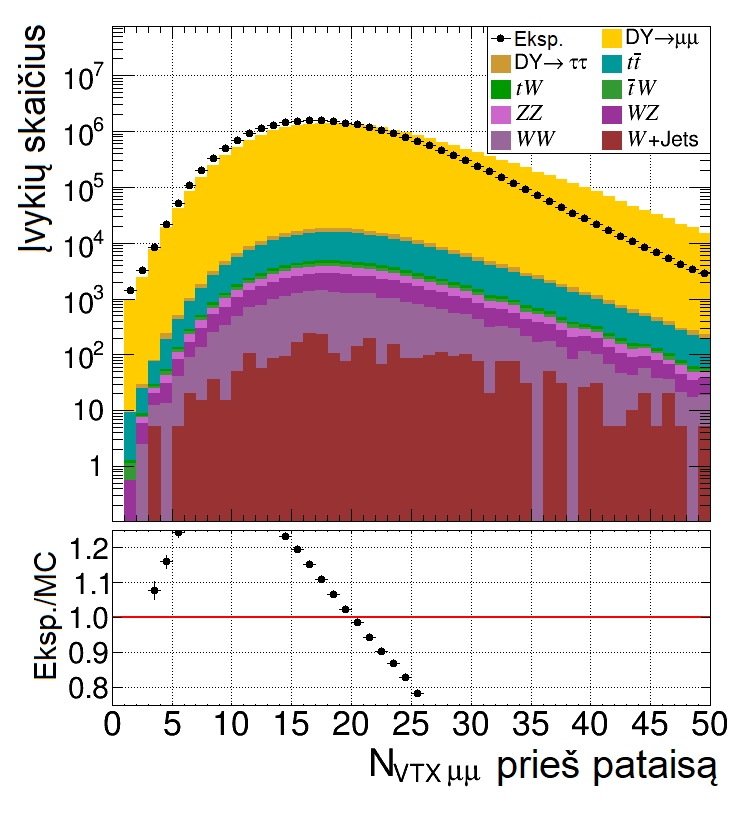
\includegraphics[width=0.48\textwidth]{Kursinis3/mumu_nVTX_before.png}
	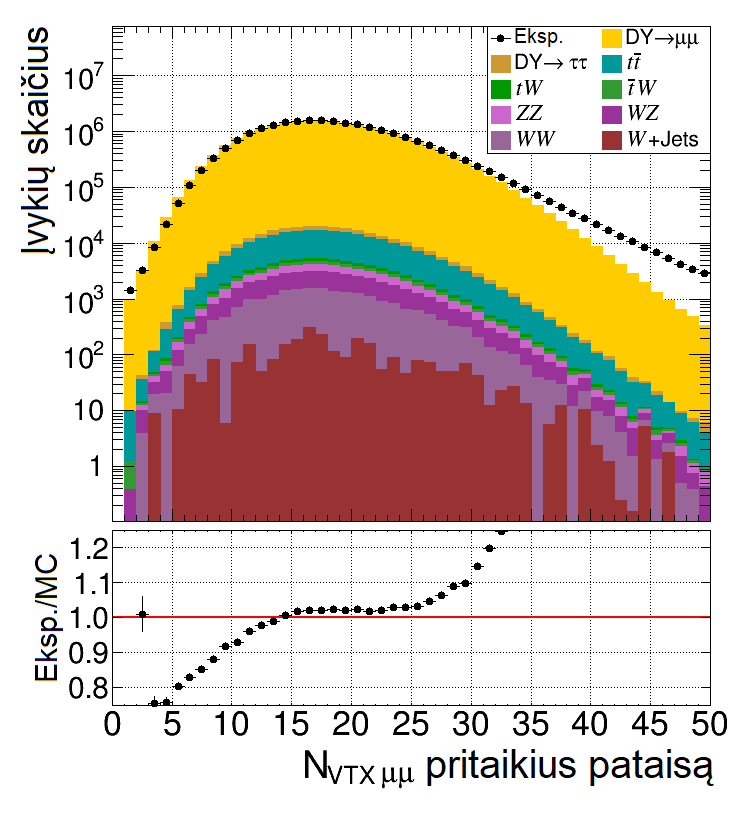
\includegraphics[width=0.48\textwidth]{Kursinis3/mumu_nVTX_after.png}
	\vspace{-0.5cm}
	\caption{\label{fig:PUba} Pirminių viršūnių skaičiaus pasiskirstymai atranką praėjusiuose įvykiuose prieš (kairėje)
		ir po (dešinėje) protonų susidūrimų tankio pataisos pritaikymo.
		Juodi taškai vaizduoja CMS detektoriumi išmatuotą, o spalvoti stulpeliai -- modeliuotus pasiskirstymus \cite{MAk2}.}
	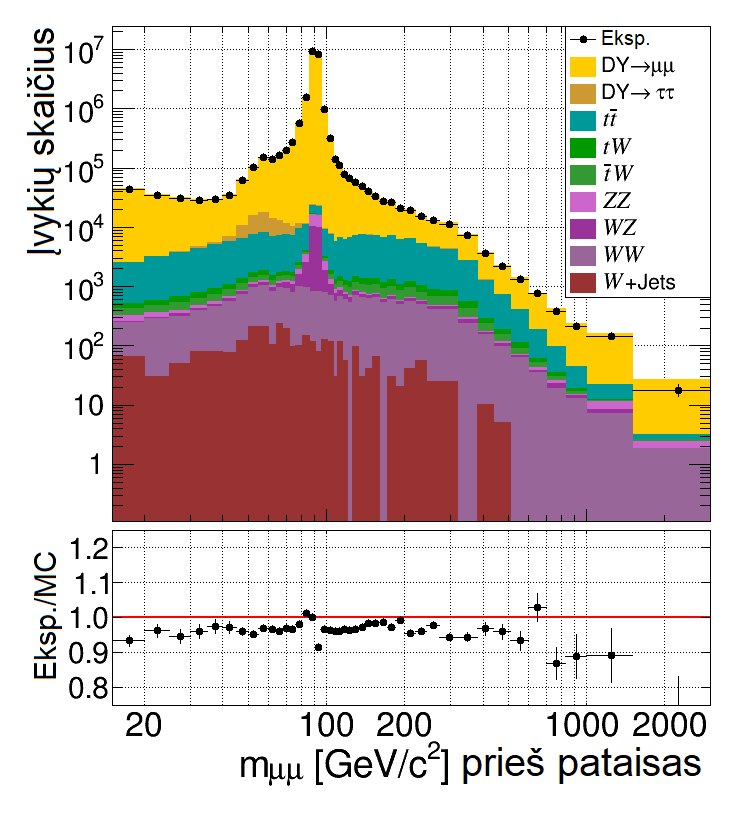
\includegraphics[width=0.48\textwidth]{Kursinis3/mumu_mass_before.png}
	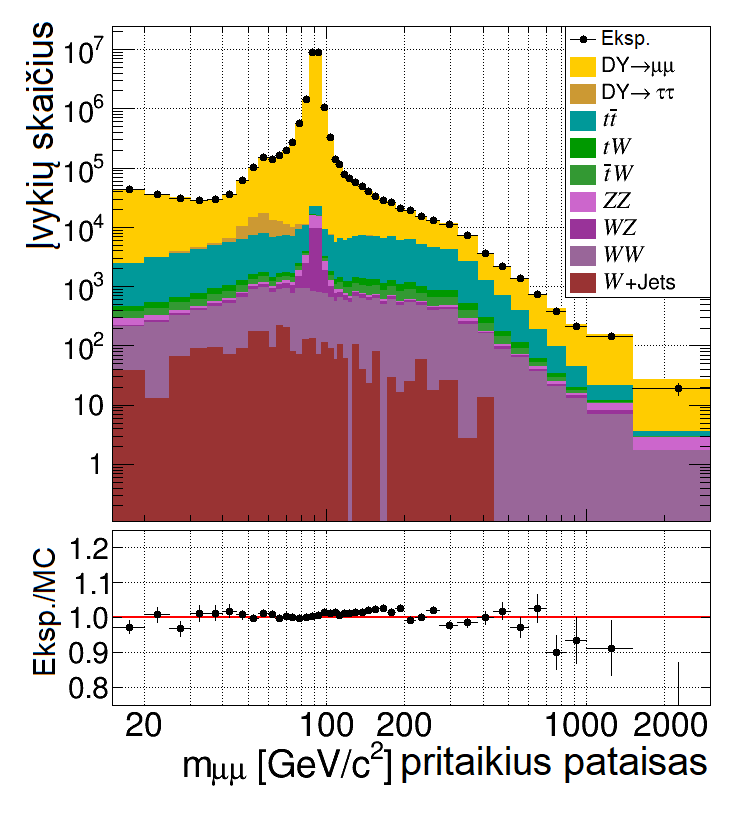
\includegraphics[width=0.48\textwidth]{Kursinis3/mumu_mass_afterSF.png}
	\vspace{-0.5cm}
	\caption{\label{fig:invMba} Miuonų porų invariantinės masės pasiskirstymai prieš ir po miuonų impulso matavimo skalės
	bei efektyvumo pataisų pritaikymo.}
\end{figure}

Matavimo ir modeliavimo rezultatų nesutapimą gali nulemti ne tik modeliavimo trūkumai, bet ir neidealios eksperimentinės sąlygos
arba eksperimentatorių klaidos.
Leptonų poros spartos pasiskirstymus paveikė dvi aplinkybės, į kurias buvo bandoma atsižvelgti pritaikant dar dvi pataisas.
Viena pataisa buvo skirta ištaisyti protonų susidūrimo vietos $z$ koordinatės ($z$ ašis eina išilgai protonų
spindulio lėkimo krypties detektoriaus centre) nesutapimą tarp matavimo ir modeliavimo.
Tai padėjo sumažinti matavimo ir modeliavimo santykio pasiskirstymuose buvusius asimetriškumus tarp teigiamų ir neigiamų leptonų
poros spartos verčių.
Antroji pataisa buvo reikalinga todėl, kad eksperimento duomenų registravimo laikotarpiu buvo susidurta su problema,
kai dėl laiko matavimo netikslumo trigerio suveikimas kartais buvo priskiriamas ne tam įvykiui, kuris iš tikrųjų jį aktyvavo, o
ankstesniam.
Dėl šio efekto dalis įdomių įvykių, kuriuose sukurtos dalelės turėjo dideles pseudospartos vertes ($|\eta|>2$) liko neįrašyti.
Imituoti šiam pernelyg ankstyvo trigerio suveikimo efektui buvo pritaikyta pataisa, kuri priskirdavo įvykiams
svorius pagal tai, kiek ir kokių įvykyje užregistruotų objektų patenka į didelių pseudospartų sritį.
Ši pataisa turėjo įtakos ir leptonų poros spartos pasiskirstymui.
Ji padėjo sumažinti modeliuotų įvykių skaičių prie didesnių spartos modulio verčių.
Tipinės pataisos vertės vienam įvykiui siekė apie $0.98$ ir mažiau, jeigu jame buvo užfiksuota objektų, kurių $|\eta|>2$.
Taip modeliuotas rezultatas buvo priartintas prie išmatuotojo.
\ref{fig:rapiba}~pav.\ pavaizduoti leptonų poros spartos pasiskirstymai prieš ir po abiejų minėtų pataisų pritaikymo.

\begin{figure}[b!]
	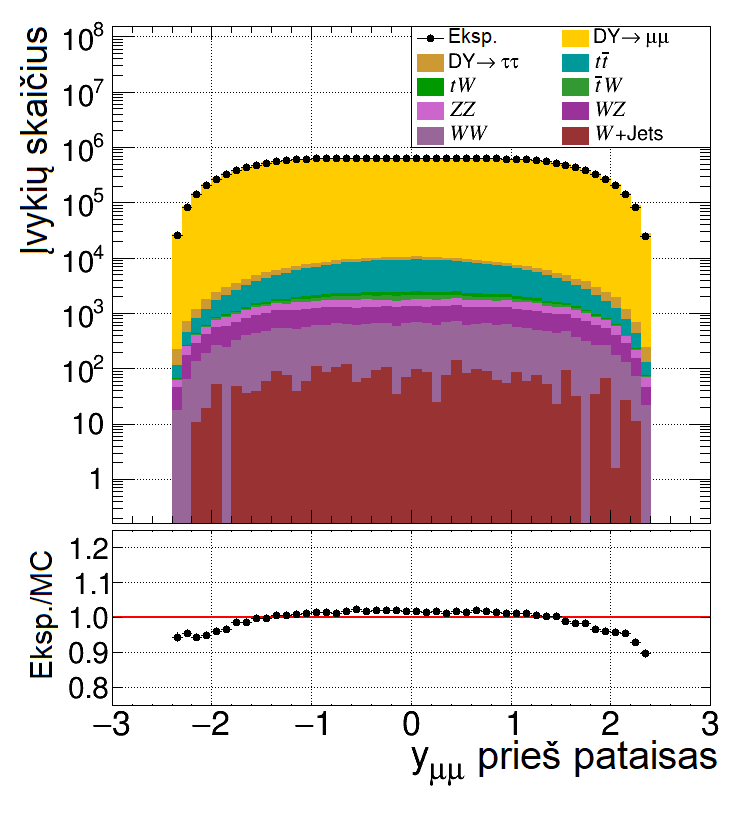
\includegraphics[width=0.48\textwidth]{Kursinis3/mumu_rapi_beforePVz.png}
	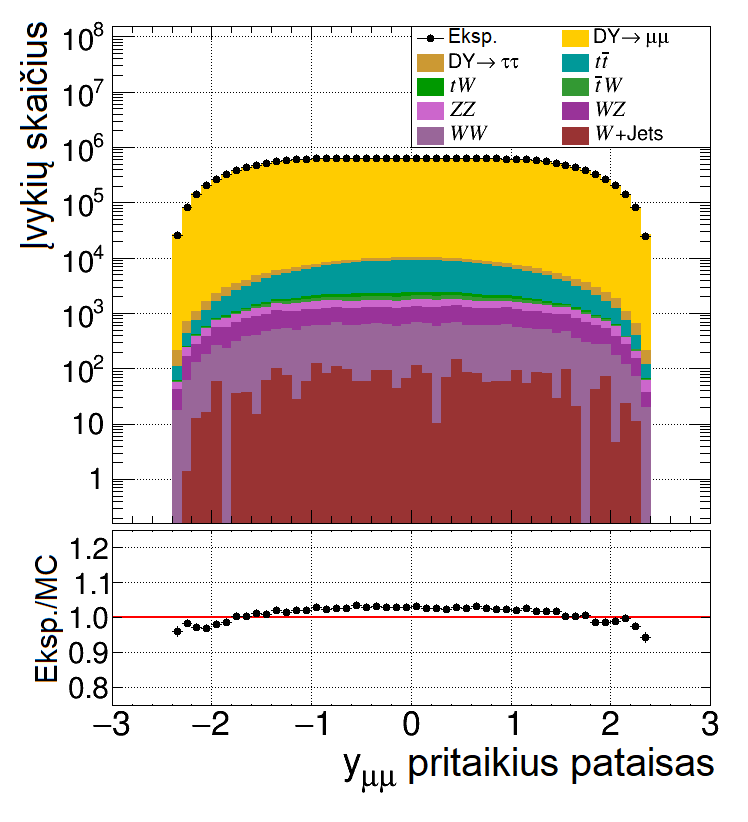
\includegraphics[width=0.48\textwidth]{Kursinis3/mumu_rapi_after.png}
	\vspace{-0.5cm}
	\caption{\label{fig:rapiba} Miuonų porų spartos pasiskirstymai prieš ir po pirminės viršūnės $z$ koordinatės bei per ankstaus
	trigerio suveikimo pataisų pritaikymo \cite{MAk2}.}
\end{figure}


\subsection{Klaidingo atpažinimo tikimybės matavimas}


\subsection{Su čiurkšlėmis susijusių triukšmo įvykių skaičiaus įvertinimas}
Fizikinio objekto klaidingo atpažinimo metodas buvo naudojamas įvertinti $\WJets$ ir $\QCD$ įvykių skaičiui.
Tai yra tokie triukšmo įvykiai, kuriuose viena arba dvi čiurkšlės buvo atpažintos, kaip miuonai.
Klaidingo atpažinimo metodas remiasi tikimybės, kad klaidingai atpažintas fizikinis objektas pateks į signalo sritį
(angliškai ši tikimybė vadinama \textit{fake rate}), įvertinimu.

Kontrolinė sritis buvo apibrėžta invertuojant miuono izoliuotumo kriterijų -- reikalaujama, kad miuono kandidato
trajektorija būtų neizoliuota nuo kitų dalelių trajektorijų (tai neretai yra čiurkšlės arba miuono, susidariusio čiurkšlėje, požymis).
Tada klaidingo atpažinimo tikimybe vadiname dydį, nusakantį, kokia dalis visų miuonais atpažintų čiurkšlių turi galimybę patekti
į signalo sritį:
\begin{equation} \label{eq:FR}
	f_{\mathrm{signal} \,| \,\mathrm{Jet}} =
	\frac{N^{\QCD}_{\mathrm{signal}}}{N^{\QCD}_{\mathrm{signal}}+N^{\QCD}_{\mathrm{control}}} \; ,
\end{equation}
čia $f_{\mathrm{signal} \,| \,\mathrm{Jet}}$ -- klaidingo atpažinimo tikimybė, $N^{\QCD}_{\mathrm{signal}}$ -- į signalo sritį
patenkančių miuonais atpažintų čiurkšlių skaičius, $N^{\QCD}_{\mathrm{control}}$ -- į kontrolinę sritį patenkančių kaip miuonai
atpažintų čiurkšlių skaičius.
Indeksas $\QCD$ žymi faktą, kad klaidingo atpažinimo tikimybės įvertinimui turėtume naudoti tik $\QCD$ įvykius, t.y., tuos
įvykius, kuriuose susidaro vien tik čiurkšlės, todėl bet koks tokiuose įvykiuose atpažintas miuonas yra kilęs iš čiurkšlės.
Vis dėlto, į kontrolinę sritį gali patekti ne vien $\QCD$, bet ir tokie įvykiai, kuriuose yra tikrų, tik dėl įvairių
priežasčių neizoliuotų miuonų.
Pavyzdžiui, dėl mažo miuono impulso laboratorinėje atskaitos sistemoje jis gali neišsiskirti.

Norint teisingai įvertinti klaidingo atpažinimo tikimybę, iš eksperimento metu užregistruotų duomenų reikėjo išskirti $\QCD$
proceso įvykius.
$\QCD$ įvykių išskyrimui buvo pasitelkti modeliuoti duomenų rinkiniai.
Paprasčiausias variantas išskirti $\QCD$ įvykius būtų iš atranką praėjusių eksperimento metu užregistruotų įvykių skaičiaus
atimti modeliuotą visų su $\QCD$ nesusijusių procesų įvykių skaičių:
\begin{equation}
	\begin{gathered}
		N^{\QCD}_{i} = N^{\mathrm{Data}}_{i} - \left( N^{\mathrm{DY}}_{i} +
		N^{\WJets}_{i} + N^{\ttbar}_{i} + N^{tW+\tbarW}_{i} +
		N^{WW+\WZ+\ZZ}_{i} \right)^{\mathrm{MC}}; \\
		\hspace{280pt} i = \mathrm{signal}, \, \mathrm{control},
	\end{gathered}
\end{equation}
tačiau šis metodas nėra tinkamas, nes pašalinių įvykių skaičius yra pakankamai didelis, o taip pat įvykiai, kuriuose leptonai
nėra izoliuoti, yra prasčiau sumodeliuoti ir ne taip gerai sutampa su matavimu.
Tikslesniam $\QCD$ įvykių skaičiaus įvertinimui buvo naudojami du skirtingi metodai:
\begin{enumerate}
	\item Santykio metodas -- $\QCD$ įvykių skaičius įvertinamas iš matavimo paėmus procentinę $\QCD$ įvykių dalį, kuri buvo apskaičiuota
	pasinaudojant modeliavimu:
	\begin{equation}
		\begin{gathered}
			N^{\QCD}_{i} = N^{\mathrm{Data}}_{i} \cdot \left(\frac{N^{\QCD}_{i}}
			{N^{\QCD}_{i} + N^{\mathrm{DY}}_{i} + N^{\WJets}_{i} +
			N^{\ttbar}_{i} + N^{tW+\tbarW}_{i} + N^{WW+\WZ+ZZ}_{i}} \right)^{\mathrm{MC}}; \\
			\hspace{300pt} i = \mathrm{signal}, \, \mathrm{control}.
		\end{gathered}
	\end{equation}
	\item Šablonų pritaikymo (angl.\ \textit{template fitting}) metodas -- $\QCD$ įvykių skaičius įvertinamas prie tam tikro
	išmatuoto pasiskirstymo pritaikius skirtingų procesų pasiskirstymų šablonus, darant prielaidą, kad įvykių tikimybinis
	pasiskirstymas yra teisingas, o normavimo amplitudė netiksli.
	Skirtingų procesų šablonai dažniausiai (ir šiame darbe) gaunami iš modeliavimo.
	Pasiskirstymas, kurio šablonai pritaikomi prie matavimo, turi būti pasirenkamas toks, kuris leistų pakankamai gerai
	atskirti $\QCD$ nuo kitų procesų (pasiskirstymų forma turėtų būti skirtinga).
	Šiuo atveju buvo naudojami miuono trajektorijos izoliuotumo pasiskirstymo šablonai.
	Turint detektoriaus išmatuotą pasiskirstymą ir skirtingų procesų šablonus, stengiamasi gauti geriausią sutapimą tarp matavimo ir
	šablonų sumos varijuojant kiekvienam šablonui priskirtus svorinius daugiklius:
	\begin{equation}
		\begin{gathered}
			N^{\mathrm{Data}}_{i}(I^{\mathrm{rel.}}_{\mathrm{PF}}) \approx
			\lambda^{\mathrm{fit}}_{\,i}\, N^{\,\QCD}_{i}(I^{\mathrm{rel.}}_{\mathrm{PF}}) +
			\epsilon^{\,\mathrm{fit}}_{\,i}\, N^{\,\mathrm{DY}}_{i}(I^{\mathrm{rel.}}_{\mathrm{PF}}) +
			\zeta^{\,\mathrm{fit}}_{\,i}\, N^{\,\WJets}_{i}(I^{\mathrm{rel.}}_{\mathrm{PF}}) + \\[7pt] +
			\theta^{\,\mathrm{fit}}_{i}\, N^{\,\ttbar}_{i}(I^{\mathrm{rel.}}_{\mathrm{PF}}) +
			\kappa^{\,\mathrm{fit}}_{\,i}\, N^{\,tW}_{i}(I^{\mathrm{rel.}}_{\mathrm{PF}}) + 
			\xi^{\,\mathrm{fit}}_{i}\, N^{\,\tbarW}_{i}(I^{\mathrm{rel.}}_{\mathrm{PF}}) +
			\tau^{\,\mathrm{fit}}_{i}\, N^{\,WW}_{i}(I^{\mathrm{rel.}}_{\mathrm{PF}}) + \\[7pt] +
			\chi^{\,\mathrm{fit}}_{\,i}\, N^{\,\WZ}_{i}(I^{\mathrm{rel.}}_{\mathrm{PF}}) +
			\psi^{\,\mathrm{fit}}_{i}\, N^{\,\ZZ}_{i}(I^{\mathrm{rel.}}_{\mathrm{PF}});
			\hspace{74pt} i = \mathrm{signal}, \, \mathrm{control}.
		\end{gathered}
	\end{equation}
	Čia $\lambda^{\mathrm{fit}}_{\,i}$, $\epsilon^{\,\mathrm{fit}}_{\,i}$ ir t.t.\ -- varijuojami daugikliai,
	kuriuos keičiant bandoma gauti geriausią šablonų sumos sutapimą su matavimu mažiausių kvadratų metodu.
	Idealiu atveju šie daugikliai turėtų būti lygūs vienetui. 
	Gavus daugiklių vertes klaidingo atpažinimo tikimybė įvertinama naudojant modeliuotą $\QCD$ įvykių skaičių, padaugintą
	iš gautojo daugiklio vertės:
	\begin{equation}
		f_{\mathrm{signal} \,| \,\mathrm{Jet}} =
		\frac{\lambda^{\mathrm{fit}}_{\,\mathrm{signal}}\, N^{\,\QCD \; \mathrm{MC}}_{\mathrm{signal}}}
		{\lambda^{\mathrm{fit}}_{\,\mathrm{signal}}\, N^{\,\QCD \; \mathrm{MC}}_{\mathrm{signal}} +
		\lambda^{\mathrm{fit}}_{\,\mathrm{control}}\, N^{\,\QCD \; \mathrm{MC}}_{\mathrm{control}}}\, .
	\end{equation}
	Svarbu atkreipti dėmesį, kad, nors šablonų pritaikymas daromas izoliuotumo pasiskirstymui, šis pasiskirstymas klaidingo
	atpažinimo tikimybėje neatsispindi: įvertindami klaidingo atpažinimo tikimybę naudojame tik gautą svorinio daugiklio vertę.
	Šablonų pritaikymo metodas yra laikomas tikslesniu nei santykio metodas, todėl jis buvo naudojamas kaip pagrindinis rezultatas.
\end{enumerate}

\subsection{Matavimo paklaidų įvertinimas}\label{sec:uncertainties}
Analizuojant protonų susidūrimus laikoma, kad įvykių skaičius yra pasiskirstęs pagal Puasono dėsnį.
Puasono pasiskirstymu aprašomo įvykių skaičiaus standartinis nuokrypis yra lygus kvadratinei šakniai iš labiausiai
tikėtino įvykių skaičiaus.
Atliekant realų eksperimentą, labiausiai tikėtinas įvykių skaičius nėra tiksliai žinomas, todėl atranką praėjusių
įvykių skaičiaus statistinio neapibrėžtumo verte laikoma kvadratinė šaknis iš užregistruoto įvykių skaičiaus.

Kai modeliuoti įvykiai turi nelygius vienetui svorius, jų skaičiaus $N$ statistinis neapibrėžtumas $(\Delta N)_{\mathrm{Stat.\,}}$
įvertinamas kaip kvadratinė šaknis iš modeliuotų įvykių svorių kvadratų sumos:
\begin{equation}
	(\Delta N)_{\mathrm{Stat.\,}} = \sqrt{\sum_{i=1}^{N}w_{i}^{2}} \; ,
	\label{eq:Sumw2Unc}
\end{equation}
čia $$w_{i}=w_{i}^{\mathrm{Norm.}} \cdot \prod_{p=1}^{N_{\mathrm{Pat.}}}w_{i}^{p} \; ,$$
kur $w_{i}^{\mathrm{Norm.}}$ -- modeliuoto įvykio normuojantis svoris, gaunamas iš \eqref{eq:NLOweight} išraiškos,
$w_{i}^{p}$ -- modeliuotam įvykiui pataisos $p$ priskirtas svorinis daugiklis, $N_{\mathrm{Pat.}}$ -- pritaikytų
skirtingų pataisų skaičius.
Modeliuotiems įvykiams taikytos pataisos yra aprašytos \ref{sec:corrections}~skyriuje.
Jeigu modeliuotų įvykių turime daugiau, nei buvo užregistruota eksperimento metu, jiems bus priskiriami mažesni už
vienetą svoriai ir sunormuoto įvykių skaičiaus statistinė paklaida bus mažesnė nei eksperimento metu užregistruotų
įvykių.
Tai yra vienas iš modeliavimo privalumų, kai modeliuojami mažo tikėtinumo įvykiai.
Tuo tarpu, kai modeliuojami labai didelio tikėtinumo įvykiai, priklausomai nuo sumodeliuoto įvykių skaičiaus
jiems gali būti priskiriami labai dideli svoriai.
Tokiu atveju statistinis įvykių skaičiaus neapibrėžtumas bus gerokai didesnis nei detektoriaus užregistruotiems įvykiams.
Tai yra vienas iš modeliavimo trūkumų ir viena iš pagrindinių priežasčių, kodėl naudojamas klaidingo atpažinimo metodas
$\QCD$ ir $\WJets$ įvykių skaičiaus įvertinimui -- jų reakcijos skerspjūviai yra labai dideli ir norint juos kokybiškai
sumodeliuoti reikia ypatingai didelių skaičiavimo resursų.
Jeigu įvykiams priskiriami vienetiniai svoriai, iš \eqref{eq:Sumw2Unc} išraiškos gauname, kad įvykių
skaičiaus paklaida lygi kvadratinei šakniai iš įvykių skaičiaus, taigi, ši formulė tinkama ir eksperimento
metu užregistruotų įvykių skaičiaus statistinio neapibrėžtumo įvertinimui.
Fizikinio objekto klaidingo atpažinimo metodu įvertinto triukšmo įvykių skaičiaus statistinis neapibrėžtumas taip
pat buvo įvertintas paimant kvadratinę šaknį iš gauto rezultato, nes klaidingo atpažinimo tikimybė yra naudojama
kaip svorinis daugiklis, kuris bendru atveju yra labai mažas, todėl neapibrėžtumas, įvertintas naudojantis
\ref{eq:Sumw2Unc} formule būtų netikroviškai mažas.

Galimiems sisteminiams nukrypimams įvertinti CMS statistikos komitetas rekomenduoja turėti bent du skirtingais būdais
atliktus matavimus, kurie, idealiu atveju, turėtų duoti sutampančius įverčius.
Kadangi tikroji vertė, kurią bandoma išmatuoti, yra nežinoma, daroma prielaida, jog skirtingi įverčiai yra
lygiaverčiai ir nepriklausomi, o tikroji vertė yra artimoje aplinkoje.
Tokiu atveju skirtumo tarp dviejų skirtingų rezultatų absoliučioji vertė yra pakankamai saugus sisteminės matavimo
paklaidos įvertis.

Šiame darbe buvo matuojamas Drell-Yan proceso triukšmo įvykių skaičius, o turimi du skirtingi įverčiai buvo gauti naudojant
skirtingas klaidingo atpažinimo tikimybės įvertinimo metodikas: santykio ir šablonų pritaikymo metodą.
Taigi, pagrindinė $\QCD$ ir $\WJets$ įvykių skaičiaus įverčio sisteminės paklaidos sudedamoji dalis buvo įvertinta pagal
tokią formulę:
\begin{equation}
	(\Delta N_{ll}^{\mathcal{P} \; \mathrm{įvert.}})_{\mathrm{Sist.\,}} =
	\left| N_{ll}^{\mathcal{P} \; \mathrm{įvert.}}(\mathrm{šabl.}) -
	N_{ll}^{\mathcal{P} \; \mathrm{įvert.}}(\mathrm{sant.}) \right| \;  ;
	\;\;\;\;\; \mathcal{P} = \QCD, \; \WJets \; ,
	\label{eq:systUncFR}
\end{equation}
čia \ltq{įvert.}\ žymi matavimu grįstą įvertį, \ltq{fit.}\ žymi klaidingo atpažinimo tikimybei įvertinti naudotą šablonų
pritaikymo metodą, o \ltq{sant.}\ -- santykio metodą.

Kadangi klaidingo atpažinimo tikimybei įvertinti buvo naudojamas baigtinis įvykių skaičius, ji turi savo statistinį neapibrėžtumą,
kuris neatsispindi galutinio triukšmo įvykių skaičiaus įverčio statistiniame neapibrėžtume.
Dėl šios priežasties klaidingo atpažinimo tikimybės statistinis neapibrėžtumas buvo įskaitomas laikant jį papildomu indėliu į
sisteminę įverčio paklaidą.
Skirtingos paklaidos dedamosios, laikant, kad jos yra tarpusavyje nepriklausomos, buvo sudedamos pagal Pitagoro teoremą.


\section{Rezultatai ir jų aptarimas}
Drell-Yan proceso triukšmo įvykių skaičius, susijęs su $\DYtau$, $t\bar{t}\,$, $WW$, $tW$, $\bar{t}W$ procesais buvo įvertintas
$\emu$ metodu ankstesniame darbe \cite{MAk2}.
Šie triukšmo įvykiai sudaro $1.06\%$ visų $\mu\mu$ įvykių.
Sisteminė $\emu$ metodo įverčio paklaida buvo įvertinta kaip skirtumo tarp modeliuoto ir $\emu$ metodo įverčio modulis, pagal
CMS statistikos komiteto rekomendacijas.
Invariantinės masės histogramų, kai naudojami vien modeliuoti įverčiai ir kai naudojamas $\emu$ metodas palyginimas pateikiamas
\ref{fig:MassMCemu}~pav.
Modeliuotų $\mu\mu$ triukšmo įvykių skaičius lygus $250500$, o įvertinus $\mu\mu$ triukšmo įvykių skaičių  $e\mu$ metodu
gauta $241105$ įvykių.
Lyginant su modeliavimu, $\emu$ metodas visoje tirtoje invariantinės masės srityje susumuotą triukšmo įvykių skaičių
sumažino maždaug $4$-ais procentais.
Abiejuose pateikiamuose grafikuose naudojami modeliuoti $\WZ$, $\ZZ$, $\WJets$ ir $\QCD$ procesų įverčiai.
Verta atkreipti dėmesį, kad modeliuoti $\WJets$ ir $\QCD$ procesų įverčiai turi netolydžius invariantinės masės pasiskirstymus:
įvykių skaičiaus skirtumai tarp gretimų histogramos stulpelių vietomis skiriasi dešimtimis kartų, daug stulpelių yra tušti
net žemų masių srityse (ypač $\QCD$ atveju).
Tai rodo prastą šių dviejų procesų modeliavimo kokybę.
$\QCD$ ir $\WJets$, lyginant su kitais Drell-Yan triukšmo procesais turi labai didelį reakcijos skerspjūvį, tačiau artimą
nuliui tikimybę praeiti Drell-Yan proceso atranką.
Sumodeliavus tiek su šiais procesais susijusių įvykių, kiek leidžia turimi skaičiavimo resursai ($2.8\cdot10^8$ $\QCD$ ir
$6.3\cdot10^8$ $\WJets$ įvykių), iš jų Drell-Yan proceso atranką praeina vos $40$ $\QCD$ ir $1288$ $\WJets$ įvykiai.
Dėl didelio reakcijos skerspjūvio šiems įvykiams priskiriami dideli svoriai, kurių vertės siekia net iki kelių tūkstančių:
sunormavus įvykius pagal išmatuotą integruotąjį šviesį buvo gauta $1673\pm1498$ $\QCD$ ir $2704pm200$ $\WJets$ įvykių. 
Tai paaiškina pasiskirstymuose matomus netolydumus ir yra pagrindinė priežastis, kodėl šių triukšmų indėlį reikia įvertinti
matavimu grįstais metodais.

\begin{figure}[b!]
	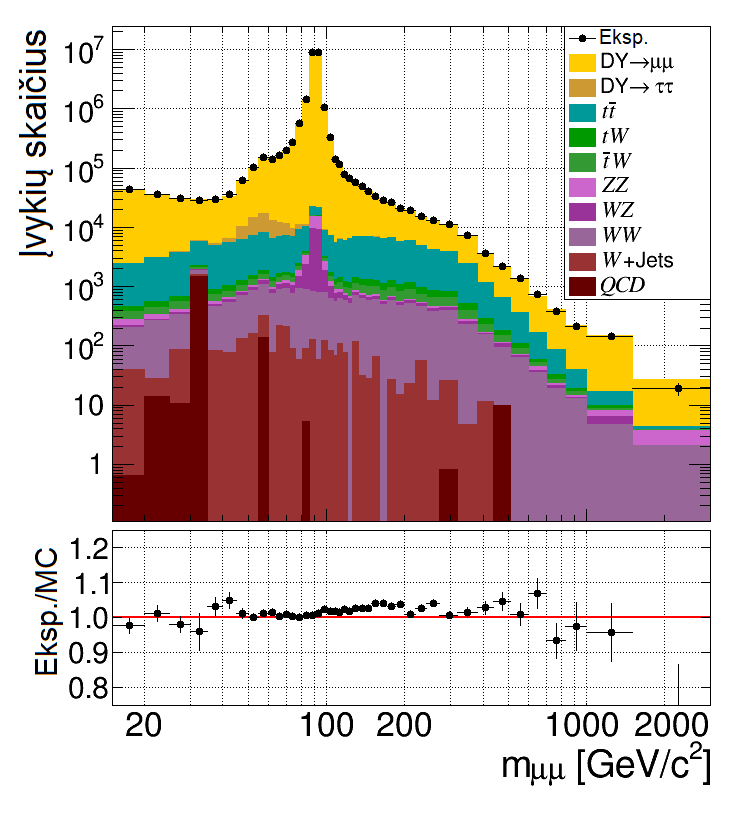
\includegraphics[width=0.49\textwidth]{Kursinis3/mumu_mass_after_wQCD.png}
	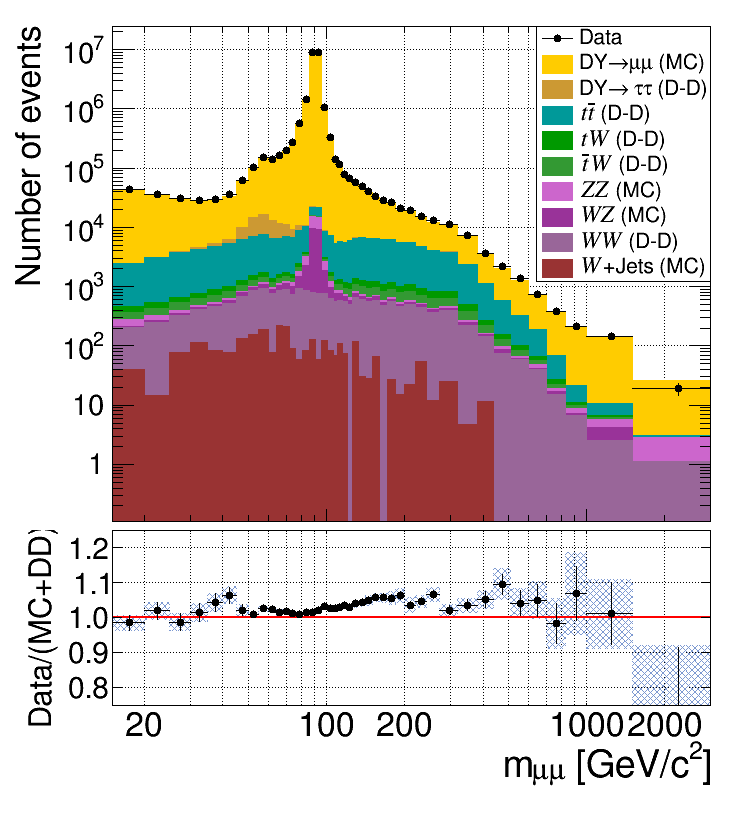
\includegraphics[width=0.49\textwidth]{Kursinis3/mumu_mass_wEMuEst.png}
	\vspace{-0.5cm}
	\caption{\label{fig:MassMCemu}
		Miuonų poros invariantinės masės pasiskirstymai pritaikius visas pataisas.
		Juodi taškai vaizduoja CMS detektoriumi išmatuotus pasiskirstymus, o spalvoti stulpeliai -- modeliuotus (kairėje)
		arba $\emu$ metodu įvertintus (dešinėje) įvykius.
		Eksperimento ir įverčio santykio grafike esančios mėlynos juostos vaizduoja sumines paklaidas.}
\end{figure}

Įvykiai klaidingo atpažinimo tikimybei įvertinti buvo atrenkami pagal \ref{table:FR}~lentelėje nurodytus atrankos kriterijus.
Drell-Yan signalo atrankoje naudoti vieno miuono trigeriai šiuo atveju buvo netinkami, nes juose yra užkoduotas ir miuono trajektorijos
izoliuotumo reikalavimas, kuris šiuo atveju buvo nereikalingas.
Dėl šios priežasties buvo pasirinktas kitas vieno miuono trigeris, kuris aktyvuojamas, kai aptinkamas miuonas su skersiniu impulsu,
viršijančiu $50$~GeV. Šis trigeris neatsižvelgia į miuono izoliuotumą.
Dėl pasikeitusio trigerio buvo naudojami ir kitokie kinematiniai reikalavimai: atrenkami miuonai su $\pT>52$~GeV.
Miuonams buvo taikomas tas pats Drell-Yan signalo atrankoje naudotas \ttt{TightID} reikalavimas.
Reikalavimai miuono krūviui ar įvykyje užregistruotų miuonų skaičiui nebuvo taikomi.
Klaidingo atpažinimo tikimybė buvo įvertinta pagal \eqref{eq:realfake} formulę keliose skirtingose miuono skersinio impulso ir
pseudospartos srityse ($f_{\mathrm{Signal} \, | \, \mathrm{Jet}}$ yra funkcija nuo $\pT$ ir $\eta$).

\begin{table}[t!]
	\begin{tabular}{|c|c|}
		\hline
		\textbf{Signalo sritis} & \textbf{Kontrolinė sritis} \\
		\hline\hline
		\multicolumn{2}{|c|}{Aukšto lygio trigeris \ttt{Mu\_50}} \\
		\hline
		\multicolumn{2}{|c|}{$\pT>52$~GeV} \\
		\hline
		\multicolumn{2}{|c|}{$|\eta|<2.4$} \\
		\hline
		\multicolumn{2}{|c|}{\ttt{TightID} reikalavimai} \\
		\hline
		$I_{\mathrm{PF}}^{\mathrm{rel.}} < 0.15$ & $I_{\mathrm{PF}}^{\mathrm{rel.}} > 0.15$ \\
		\hline
	\end{tabular}
	\caption{\label{table:FR} Naudoti miuonų atrankos kriterijai signalo ir kontrolinei sritims. Visi kriterijai, išskyrus vieną
	abiem sritims yra vienodi.}
\end{table}

\begin{figure}[b!]
	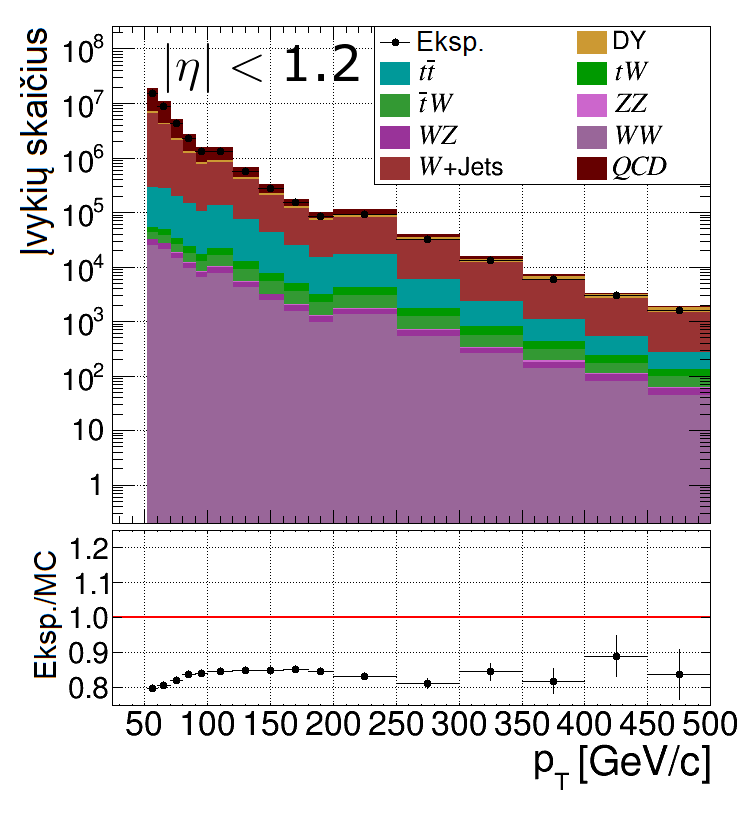
\includegraphics[width=0.48\textwidth]{Kursinis3/FRest_pT_deno_barrel.png}
	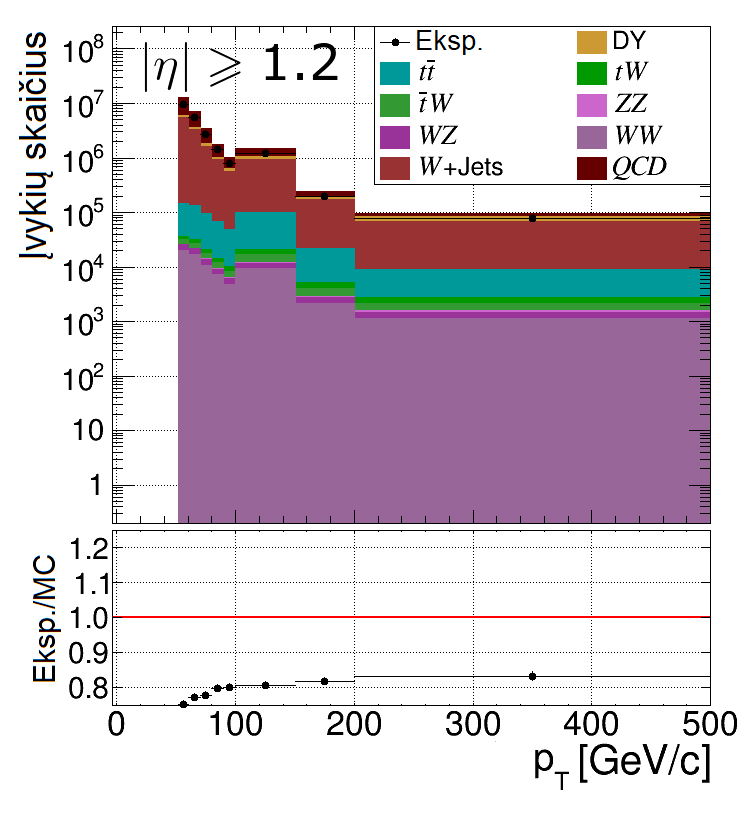
\includegraphics[width=0.48\textwidth]{Kursinis3/FRest_pT_deno_endcap.png}
	\vspace{-0.5cm}
	\caption{\label{fig:jet_pT_before}
		Klaidingo atpažinimo tikimybės įvertinimui atliktą įvykių atranką praėjusių miuonų kandidatų skersinių impulsų
		pasiskirstymai, kai miuonas pataiko į detektoriaus cilindrinę (kairėje) ir antgalio (dešinėje) dalį.
		Dėl nepakankamai tikslaus modeliavimo, jo sutapimas su eksperimento rezultatu yra prastas.}
\end{figure}

\begin{figure}[p!]
	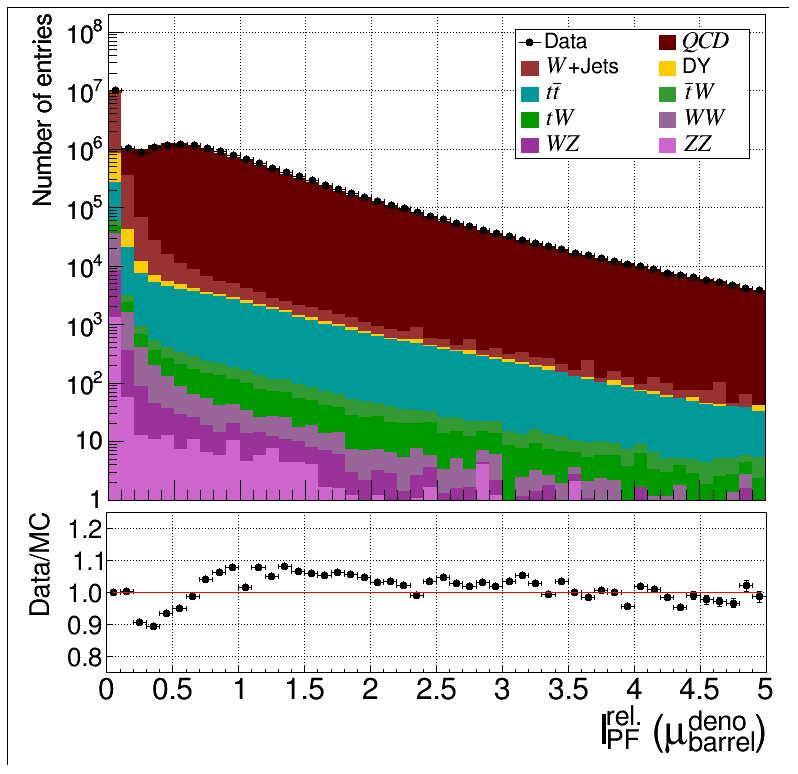
\includegraphics[width=0.45\textwidth]{Kursinis3/TFit_DB_50to70.png}
	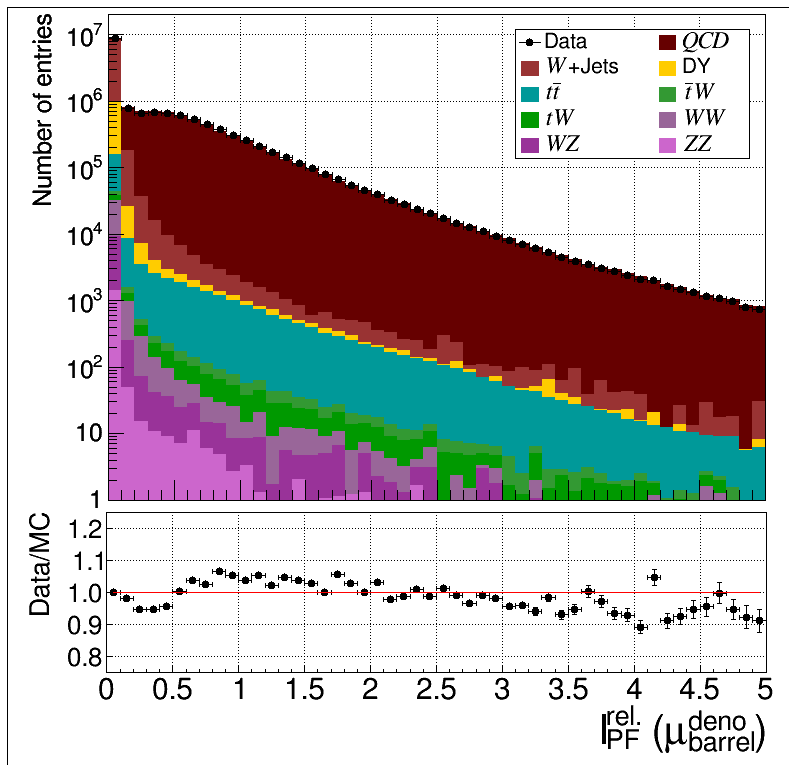
\includegraphics[width=0.45\textwidth]{Kursinis3/TFit_DE_50to70.png}
	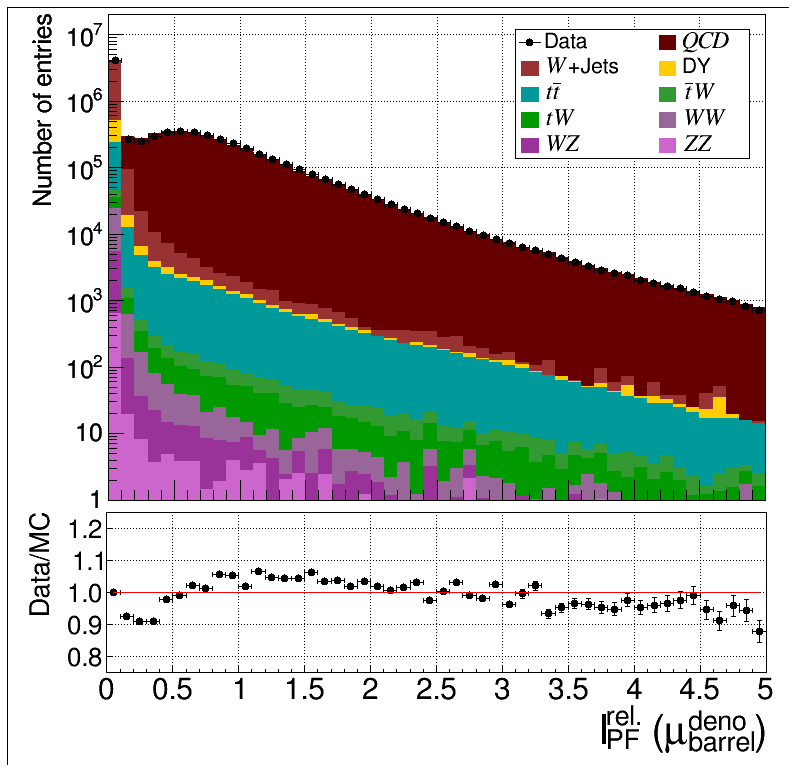
\includegraphics[width=0.45\textwidth]{Kursinis3/TFit_DB_70to100.png}
	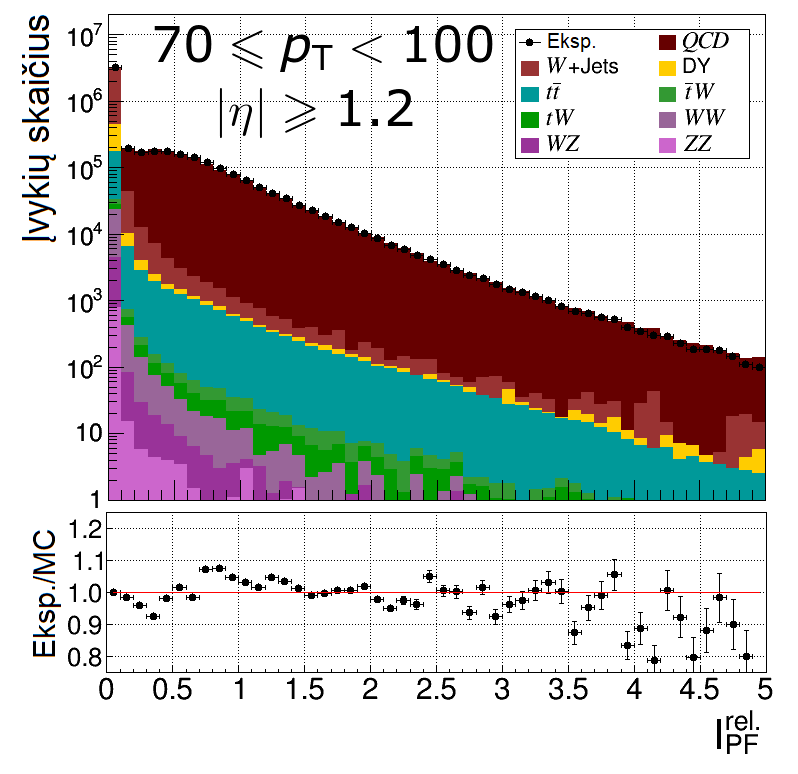
\includegraphics[width=0.45\textwidth]{Kursinis3/TFit_DE_70to100.png}
	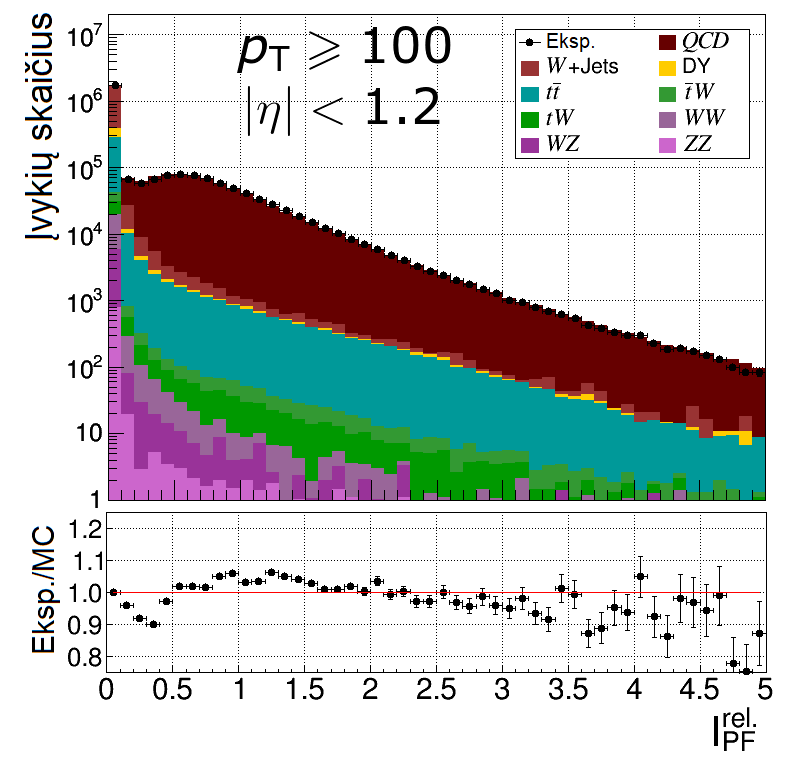
\includegraphics[width=0.45\textwidth]{Kursinis3/TFit_DB_100to500.png}
	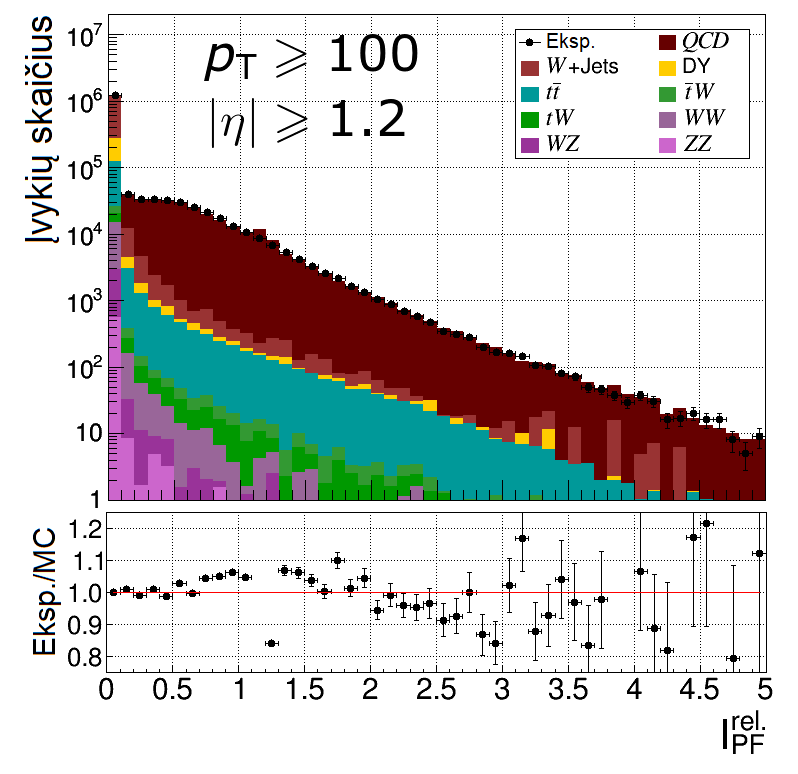
\includegraphics[width=0.45\textwidth]{Kursinis3/TFit_DE_100to500.png}
	\vspace{-0.2cm}
	\caption{\label{fig:templateFit}
		Eksperimentiniai miuono trajektorijos izoliuotumo pasiskirstymai detektoriaus cilindrinėje (kairėje)
		ir  antgalių (dešinėje) dalyse, bei prie jų pritaikyti modeliuoti šablonai.
		Iš viršaus į apačią pavaizduoti pasiskirstimai miuonų kandidatams, kurių $\pT\in(52, 70)$~GeV,
		$\pT\in[70, 100)$~GeV ir $\pT\in[100, 500)$~GeV.}
\end{figure}

\ref{fig:jet_pT_before}~pav.\ pavaizduoti atranką praėjusių miuonų skersinio impulso pasiskirstymai.
Dėl nepakankamai tikslaus modeliavimo nesutapimas tarp eksperimento ir modeliavimo siekia $20\%$.
Dėl šios priežasties buvo laikoma, jog klaidingo atpažinimo tikimybės įvertinimas naudojant santykio metodą gali būti
nepakankamai teisingas.
Kokybiškesnį įvertinimą buvo tikimasi gauti naudojant šablonų pritaikymo metodą.
Jis buvo atliekamas prie matavimo pritaikant modeliuotus miuono trajektorijos izoliuotumo pasiskirstymus.
Izoliuotumo pasiskirstymai buvo padalinti į šešias sritis: pirmiausia dalinama į dvi dalis pagal miuono pseudospartą
($|\eta|<1.2$ atitinka miuonus, pataikiusius į detektoriaus cilindrinę dalį, o $|\eta|\geqslant 1.2$ -- į antgalių segmentus)
bei į tris dalis pagal miuono skersinį impulsą ($\pT\in(52, 70)$~GeV, $\pT\in[70, 100)$~GeV ir $\pT\in[100, 500)$~GeV).
Prie išmatuotų izoliuotumo pasiskirstymų pritaikyti šablonai pavaizduoti \ref{fig:templateFit}~pav.
Iš šablonų pritaikymo gautos normavimo daugiklio vertės $\QCD$ pasiskirstymams siekė $0.72$-$0.75$ cilindrinėje detektoriaus
srityje ir $0.60$-$0.66$ antgalių srityje.
Šablonų pritaikymas pakoregavo modeliuotų pasiskirstymų normavimą taip, kad nesutapimas tarp matavimo ir modeliavimo
sumažėjo iki $5\%$.
Pernormuoti miuonų skersinio impulso pasiskirstymai pavaizduoti \ref{fig:jet_pT_after}~pav.
Klaidingo atpažinimo tikimybė buvo įvertinta skirtingose miuono skersinio impulso srityse bei dviejose pseudospartos srityse
(atitinkančiose detektoriaus cilindro ir antgalių segmentus) naudojantis \ref{eq:FR} formule.
Klaidingo atpažinimo tikimybės vertės, gautos naudojant santykio ir šablonų pritaikymo metodus, pavaizduotos \ref{fig:FR}~pav.
Šablonų pritaikymo metodu gautos klaidingo atpažinimo tikimybės vertės yra beveik $10\%$ didesnės, už įvertintas
santykio metodu.
Čiurkšlėms, pataikiusioms į cilindrinę detektoriaus dalį, klaidingo atpažinimo tikimybė kinta apytiksliai nuo $5\%$ iki $20\%$,
o pataikiusioms į detektoriaus antgalį ji yra vidutiniškai $2.5$ karto didesnė ir kinta
apytiksliai nuo $14\%$ iki $32\%$.

\begin{figure}[p!]
	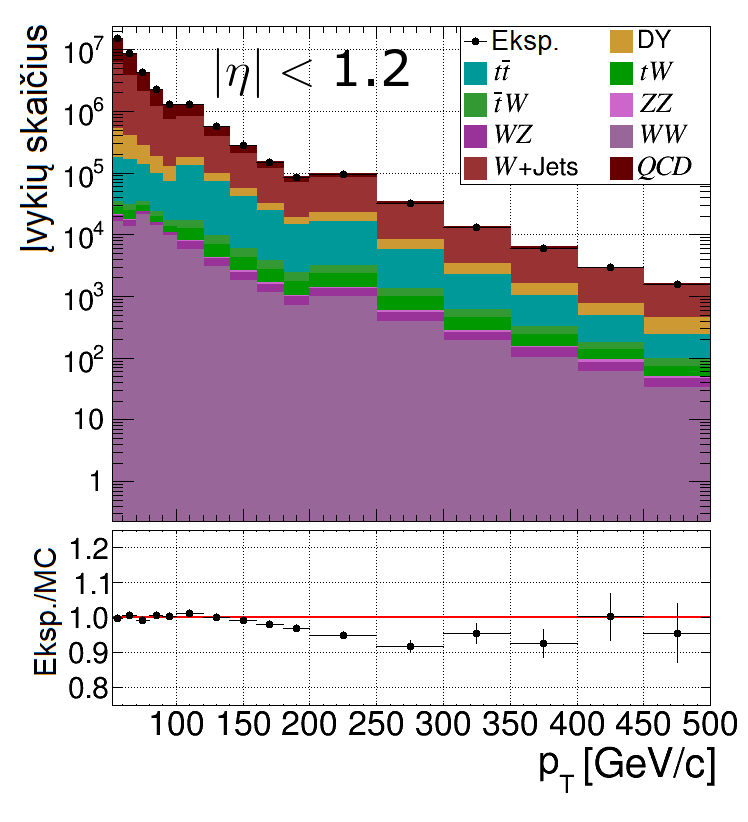
\includegraphics[width=0.48\textwidth]{Kursinis3/FRfit_pT_deno_barrel.png}
	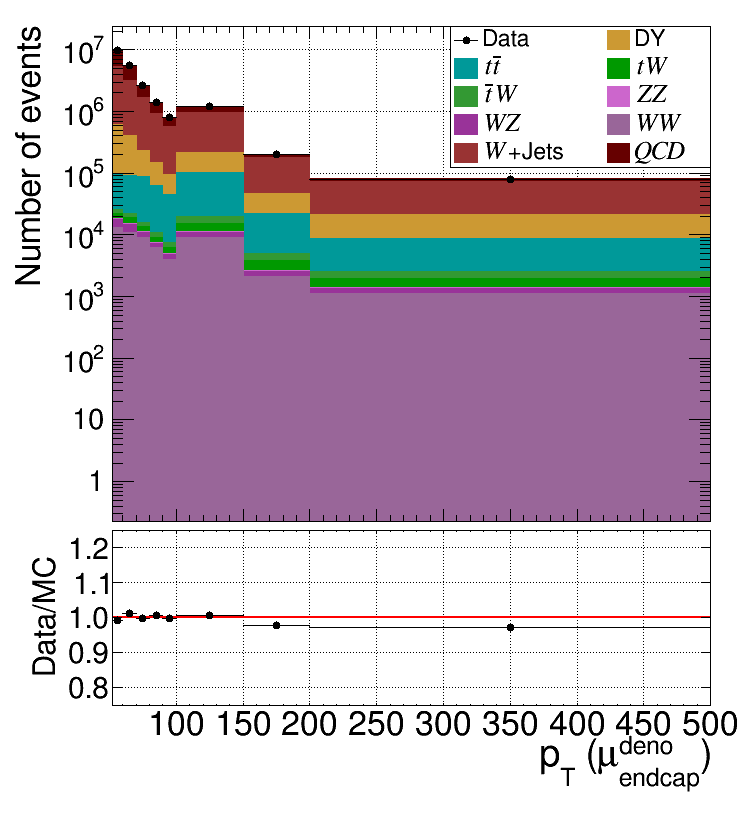
\includegraphics[width=0.48\textwidth]{Kursinis3/FRfit_pT_deno_endcap.png}
	\vspace{-0.4cm}
	\caption{\label{fig:jet_pT_after}
		Klaidingo atpažinimo tikimybės įvertinimui atliktą įvykių atranką praėjusių miuonų kandidatų skersinių impulsų
		pasiskirstymai, kai miuonas pataiko į detektoriaus cilindrinę (kairėje) ir antgalio (dešinėje) dalį.
		Šiuose grafikuose modeliuoti pasiskirstymai (parodyti \ref{fig:jet_pT_before}~pav.)\ yra pernormuoti, kad
		atitiktų iš šablonų pritaikymo gautas vertes.}
\end{figure}

\begin{figure}[p]
	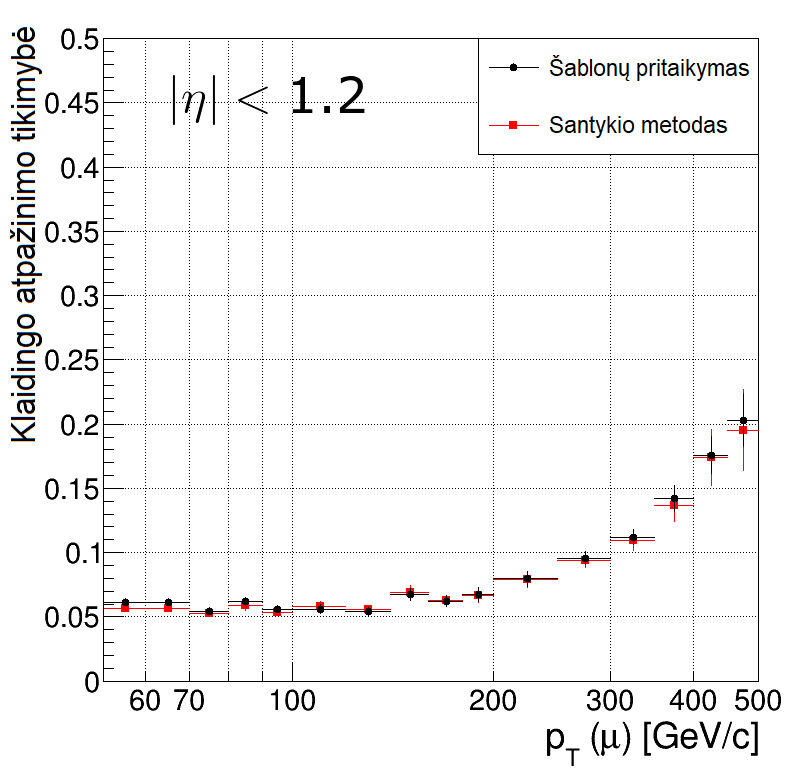
\includegraphics[width=0.48\textwidth]{Kursinis3/FR_barrel.png}
	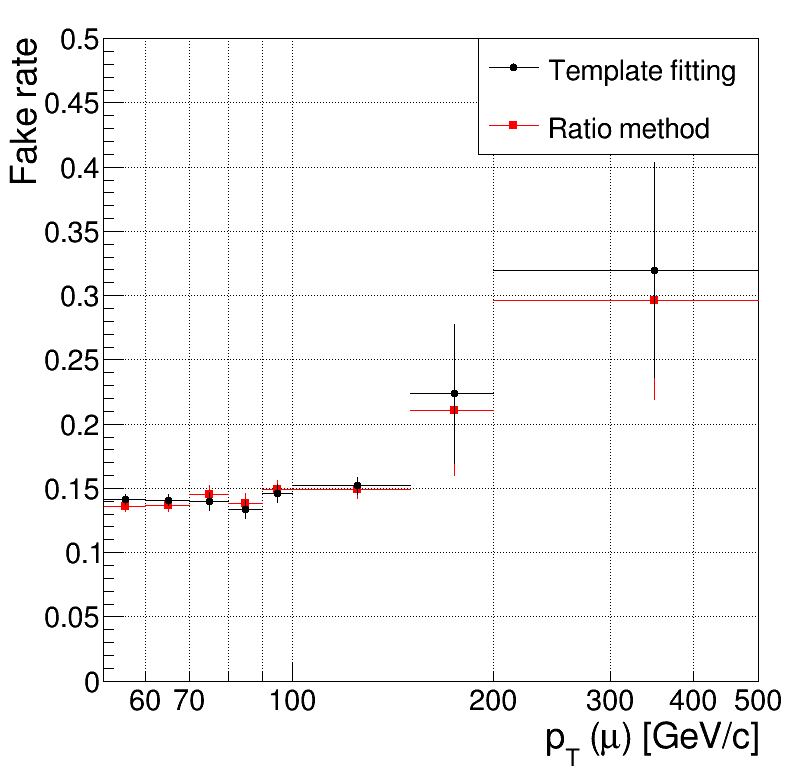
\includegraphics[width=0.48\textwidth]{Kursinis3/FR_endcap.png}
	\vspace{-0.3cm}
	\caption{\label{fig:FR}
		Apskaičiuota klaidingo atpažinimo tikimybė skirtingose skersinio impulso srityse.
		Kairėje pateiktas rezultatas trajektorijoms, einančioms per detektoriaus cilindrinę, o dešinėje -- per antgalių dalis.
		Skirtingos spalvos vaizduoja skirtingais metodais įvertintą tikimybę (žr.~legendą).}
\end{figure}

Apskaičiuota klaidingo atpažinimo tikimybė buvo panaudota įvertinant Drell-Yan proceso triukšmo įvykių skaičių, susijusį su
$\QCD$ ir $\WJets$ procesais.
Šių triukšmo įvykių skaičiaus įvertinimui buvo vykdoma atranka, kurios kriterijai nurodyti \ref{table:jetSelection}~lentelėje.
Praktiškai visi taikyti atrankos kriterijai buvo identiški Drell-Yan signalo atrankos kriterijams, nurodytiems
\ref{table:selection}~lentelėje, tačiau vienam arba dviems miuonams buvo taikomi invertuoti trajektorijos izoliuotumo
reikalavimai (atitinkamai $\WJets$ arba $\QCD$ atrankoje).
Taip pat šiuo atveju nebuvo naudojamas joks aukšto lygio trigeris (naudotas tik pirmo lygio vieno miuono trigeris, kuris
ir taip buvo naudojamas visoje atliktoje analizėje), nes, norint teisingai įvertinti triukšmo įvykių skaičių
svarbu, kad taikomi kinematiniai reikalavimai atitiktų naudojamus pagrindinėje analizėje.
To nebūtų įmanoma padaryti naudojant klaidingo atpažinimo tikimybės įvertinimui naudotą trigerį \ttt{Mu\_50},
o pagrindinės analizės trigeriai taip pat buvo netinkami dėl jau minėto reikalavimo miuonų izoliuotumui.
Smarkaus skaičiavimo laiko išaugimo dėl aukšto lygio trigerio nenaudojimo buvo išvengta iškart atmetant visus įvykius,
kuriuose nebuvo užfiksuota bent dviejų miuonų.

\begin{table}[b!]
	\begin{tabular}{|c|c|}
		\hline
		\textbf{$\WJets$ atranka} & \textbf{$\QCD$ atranka} \\
		\hline\hline
		\multicolumn{2}{|c|}{Trigeris: pirmo lygio \ttt{SingleMuon} trigeris, jokio aukšto lygio trigerio} \\
		\hline
		\multicolumn{2}{|c|}{$p_{\mathrm{T \, 1}} > 28$~GeV, $p_{\mathrm{T \, 2}} > 17$~GeV} \\
		\hline
		\multicolumn{2}{|c|}{$|\eta_1| < 2.4$, $|\eta_2| < 2.4$} \\
		\hline
		\multicolumn{2}{|c|}{\ttt{TightID} reikalavimai} \\
		\hline
		\multicolumn{2}{|c|}{\multirow{2}{37em}{\centering Pasirenkami 2 miuonai, kuriuos galima tiksliausiai suvesti į vieną
		pirminę viršūnę su $\chi^2<20$}} \\
		\multicolumn{2}{|c|}{} \\
		\hline
		\multicolumn{2}{|c|}{Priešingi elektriniai krūviai} \\
		\hline
		\multicolumn{2}{|c|}{Plokštuminis kampas $< \pi - 0.005$ rad} \\
		\hline
		\multirow{1}{22em}{\centering Vienam miuonui $I_{\mathrm{PF}}^{\mathrm{rel.}}<0.15$,
			kitam -- $I_{\mathrm{PF}}^{\mathrm{rel.}}\geqslant 0.15$} &
			\multirow{1}{15em}{\centering Abiems miuonams $I_{\mathrm{PF}}^{\mathrm{rel.}}\geqslant 0.15$} \\
		\hline
	\end{tabular}
	\caption{\label{table:jetSelection}Apibendrinti $\WJets$ ir $\QCD$ įvykių atrankos kriterijai. Indeksai $1$ ir $2$ žymi
	atitinkamai greitesnįjį ir lėtesnįjį miuoną. Šios dvi atrankos skiriasi tik vienu kriterijumi.}
\end{table}

$\QCD$ įvykių skaičius iš kontrolinės į signalo sritį buvo perkeliamas atranką praėjusiems įvykiams pritaikius svorinius
daugiklius, apskaičiuojamus pagal \ref{eq:FRapply} formulę.
\ref{fig:FR}~pav.\ pavaizduoti klaidingo atpažinimo tikimybės priklausomybės nuo skersinio impulso grafikai tampa
plokšti mažų skersinių impulsų srityse, todėl atranką praėjusiems miuono kandidatams su $\pT<52$~GeV, buvo pritaikomi
tokie patys svoriniai daugikliai, kaip ir kandidatams su $\pT=52$~GeV.
Sisteminė įverčio paklaida buvo įvertinta pagal \ref{eq:systUncFR} formulę.
\ref{fig:QCDselection}~pav.\ pateiktas atranką praėjusių į signalo sritį perkeltų miuonų porų pasiskirstymas.
Modeliavimas sufleruoja, kad tokią įvykių atranką praeina ne tik $\QCD$ proceso įvykiai, tačiau pašaliniai įvykiai
sudaro tik apie $25\%$ viso įvykių skaičiaus.
$\QCD$ įvykių skaičius buvo gautas iš eksperimento metu išmatuoto pasiskirstymo atėmus modeliuotus pasiskirstymus.
Įverčio rezultatas pavaizduotas \ref{fig:QCDest}~pav.
Įvertintas su $\QCD$ procesu susijusių Drell-Yan proceso triukšmo įvykių skaičius yra $2884\pm 54 \pm 383$:
$1.7$ karto daugiau, nei buvo įvertinta iš modeliavimo.

\begin{figure}[b!]
	\RawFloats
	\begin{minipage}{0.48\textwidth}
		\vspace{-0.8cm}
		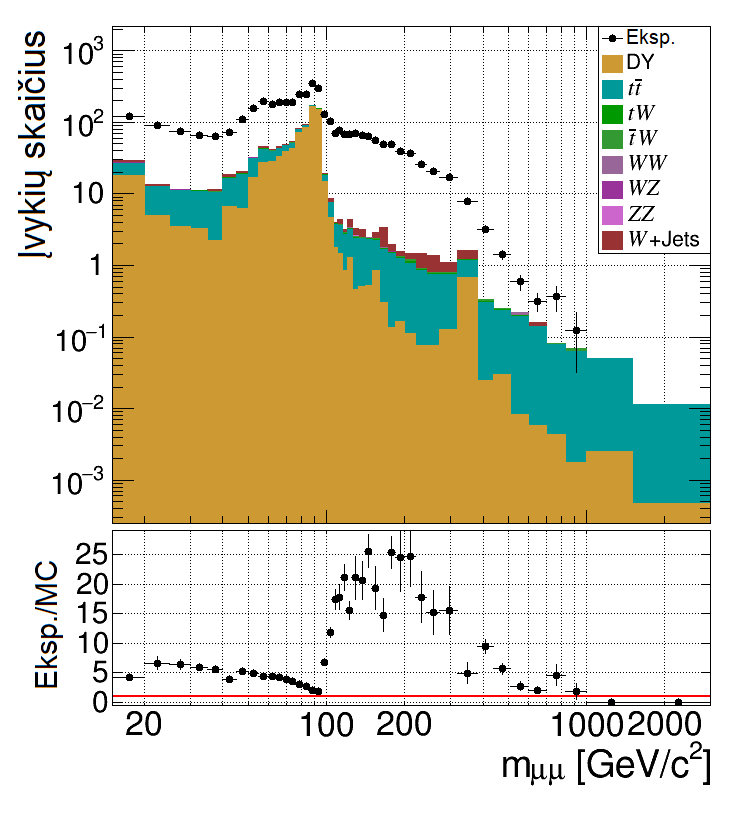
\includegraphics[width=0.95\textwidth]{Kursinis3/QCDest_subtract.png}
		\vspace{-0.53cm}
		\caption{\label{fig:QCDselection}
			$\QCD$ įvykių atranką praėjusių į signalo sritį perkeltų miuonų kandidatų porų invariantinės masės pasiskirstymas.
			Spalvotais stulpeliais pavaizduoti perkelti modeliuoti su $\QCD$ procesu nesusiję pasiskirstymai, kurie buvo atimami iš
			išmatuotojo pasiskirstymo.
		}
	\end{minipage}
	\hfill
	\begin{minipage}{0.48\textwidth}
		\vspace{-0.5cm}
		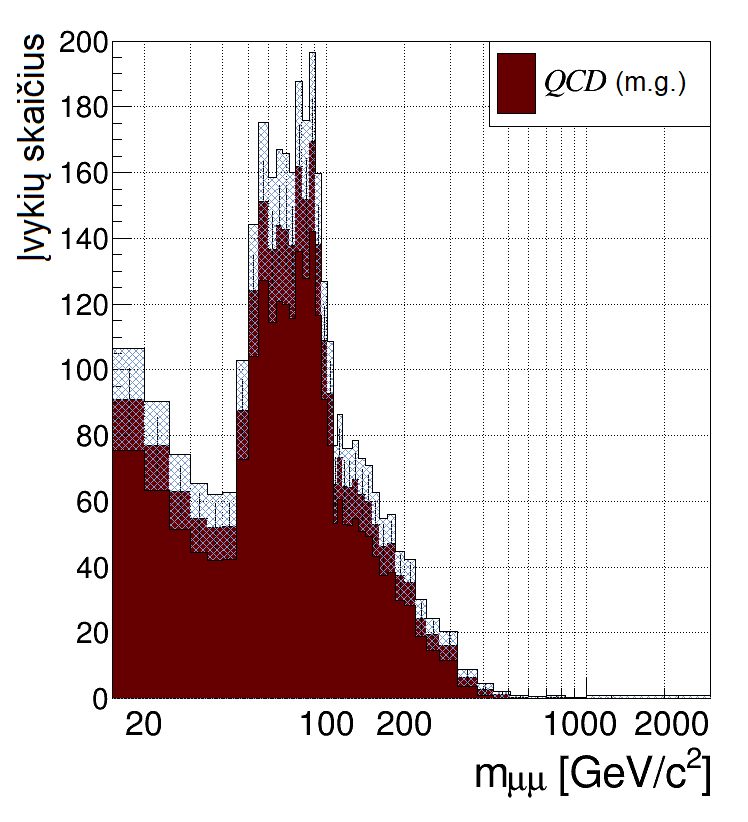
\includegraphics[width=0.95\textwidth]{Kursinis3/QCDest.png}
		\vspace{-0.35cm}
		\caption{\label{fig:QCDest}
			Klaidingo atpažinimo metodu įvertintas $\QCD$ proceso indėlis į Drell-Yan proceso atranką praeinančių miuonų
			porų invariantinės masės pasiskirstymą. Mėlynos juostos žymi sumines paklaidas. Legendoje esantis užrašas \ltq{m.g.}
			žymi faktą, jog tai yra matavimu grįstas įvertis.
		}
	\end{minipage}
	
	\begin{minipage}{0.48\textwidth}
		\vspace{-0.9cm}
		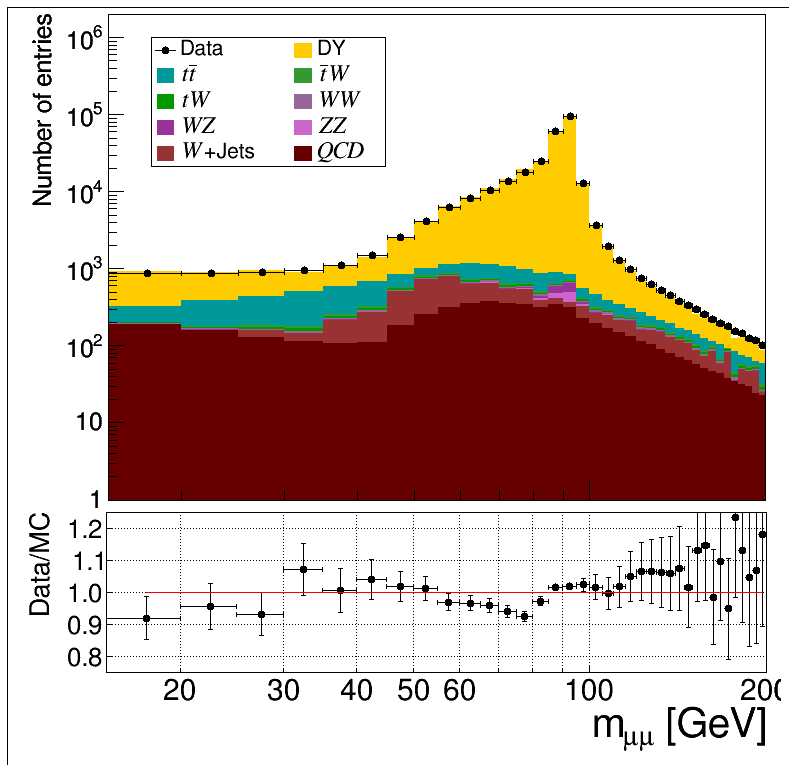
\includegraphics[width=0.98\textwidth]{Kursinis3/TFit_WJETS.png}
		\vspace{-0.4cm}
		\captionof{figure}{\label{fig:TFit_WJets}
			$\WJets$ įvykių atranką praėjusių į signalo sritį perkeltų miuonų kandidatų porų invariantinės masės pasiskirstymas
			bei prie jo pritaikyti skirtingų procesų šablonai.
		}
	\end{minipage}
	\hfill
	\begin{minipage}{0.48\textwidth}
		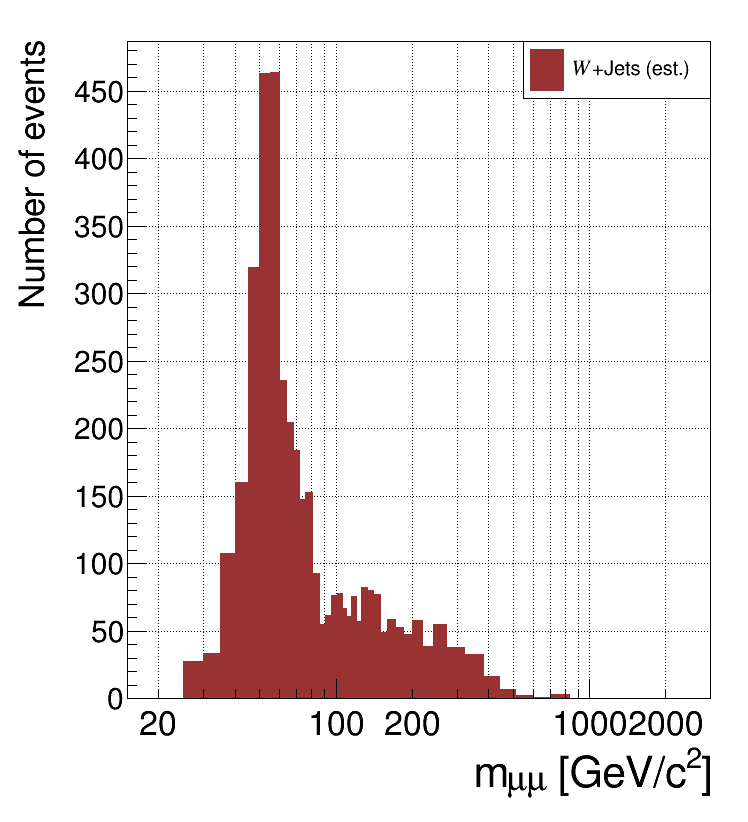
\includegraphics[width=0.9\textwidth]{Kursinis3/WJETSest.png}
		\vspace{-0.4cm}
		\captionof{figure}{\label{fig:WJetsEst}
			Klaidingo atpažinimo metodu įvertintas $\WJets$ proceso indėlis į Drell-Yan proceso atranką praeinančių miuonų
			porų invariantinės masės pasiskirstymą. Mėlynos juostos žymi sumines paklaidas, \ltq{m.g.} žymi, jog tai yra
			matavimu grįstas įvertis.
		}
	\end{minipage}
\end{figure}

$\WJets$ įvykių skaičius iš kontrolinės į signalo sritį buvo perkeliamas atranką praėjusiems įvykiams pritaikius svorinius
daugiklius pagal \ref{eq:FRapply} formulę.
Skirtingai nei $\QCD$ atranką, $\WJets$ atranką praeina didelė dalis pašalinių procesų: net $84.5\%$ visų įvykių yra
nesusiję su $\WJets$.
Modeliavimas sufleruoja, kad didžiausią indėlį į įvykių skaičių turi Drell-Yan ir $\ttbar$ procesai.
Tokiu atveju iš išmatuotojo pasiskirstymo atimti modeliuotą nėra tinkama procedūra, tad $\WJets$ pasiskirstymas buvo
gautas pasinaudojus šablonų pritaikymu.
Šiuo atveju šablonai buvo pritaikomi prie į signalo sritį perkeltų $\WJets$ atranką praėjusių miuonų porų invariantinės
masės pasiskirstymo.
$\WJets$ pasiskirstymo šablonas buvo gautas iš $\WJets$ atranką praėjusių vienodo krūvio miuonų pasiskirstymo,
kuris yra mažiau užterštas Drell-Yan proceso įvykiais.
Vienodo krūvio $\WJets$ pasiskirstymą galima naudoti kaip šabloną priešingo krūvio pasiskirstymui, nes čiurkšlėje įmanoma pagaminti
bet kokio krūvio miuoną ir vidutinė proceso kinematika nuo miuono krūvio neturėtų priklausyti.
Turėtų skirtis tik šių procesų tikimybės, tad tikimasi, jog pasiskirstymai bus apytiksliai vienodos formos, bet turės skirtingą
suintegruotą įvykių skaičių.
Iš modeliavimo buvo įvertinta, kad priešingo krūvio $\WJets$ įvykiai yra maždaug 3 kartus dažnesni, nei vienodo krūvio,
o jų pasiskirstymų forma yra panaši.
$\QCD$ proceso šablonas buvo gautas panaudojant klaidingo atpažinimo metodu įvertintą $\QCD$ pasiskirstymą.
Kitiems procesams buvo naudojami modeliuoti šablonai.

Šablonų pritaikymo rezultatas yra pateiktas \ref{fig:TFit_WJets}~pav.
Šablonų pritaikymas buvo atliktas tik iki $200$~GeV siekiančioje invariantinės masės srityje, nes prie aukštesnių
masių naudoti pasiskirstymai turi labai didelį statistinį išsibarstymą.
Gautas $\WJets$ įvykių skaičius yra lygus $3573 \pm 60 \pm 283$: $1.3$ karto daugiau, nei buvo įvertinta iš modeliavimo.
Tai yra $2.6$ kartų daugiau, nei vienodo krūvio įvykių skaičius.
Su $\WJets$ procesu susijusių triukšmo įvykių indėlio įvertis pavaizduotas \ref{fig:WJetsEst}~pav.
Lyginti klaidingo atpažinimo metodu gautus triukšmo įvykių pasiskirstymus su modeliuotais atitinkamų procesų įverčiais
nėra didelės prasmės, nes modeliuoti šių procesų pasiskirstymai yra smarkiai netolydūs dėl prastos statistikos.
Atkreiptinas dėmesys, jog tiek $\QCD$, tiek $\WJets$ įverčio sisteminės paklaidos yra ganėtinai didelės -- sudaro
reikšmingą dalį viso įvertinto įvykių skaičiaus ($13\%$ $\QCD$ atveju ir $7.4\%$ $\WJets$ atveju) bei kelis kartus
viršija statistines paklaidas ($7$ kartus $\QCD$ atveju ir $4.6$ karto $\WJets$ atveju).
Taip yra dėl to, jog įvertintas įvykių skaičius yra ganėtinai jautrus klaidingo atpažinimo tikimybės įvertinimo tikslumui
(ypatingai $\QCD$ įvykiams, kur klaidingo atpažinimo tikimybė taikoma du kartus).
Nepaisant to, toks įvertis yra gerokai kokybiškesnis už modeliuotą, kur vien statistinės paklaidos sudaro
didesnę dalį įvykių skaičiaus (net $90\%$ $\QCD$ atveju ir $8\%$ $\WJets$ atveju), o patys modeliuoti pasiskirstymai yra netolydūs.

Eksperimento metu išmatuoto Drell-Yan proceso atranką praėjusių miuonų porų invariantinių masių pasiskirstymo palyginimas
su susumuotais skirtingų procesų įverčiais, iš kurių tik $\WZ$ ir $\ZZ$ yra modeliuoti, yra pateiktas \ref{fig:MassFinal}~pav.
Lyginant su \ref{fig:MassMCemu}~pav.\ pateiktu grafiku, į kurį neįtraukti fizikinio objekto klaidingo atpažinimo metodo
įverčiai, sutapimas tarp matavimo ir įverčio pagerėjo $0.02\%$.
Nors pagerėjimas atrodo labai mažas, tačiau su čiurkšlėmis susiję atranką praėję įvykiai sudaro tik $0.03\%$ visų įvykių.
Beveik visi šie įvykiai prisideda prie matavimo ir įverčio sutapimo pagerėjimo, taigi fizikinio objekto klaidingo
atpažinimo metodo taikymas buvo naudingas.

\begin{figure}[H]
	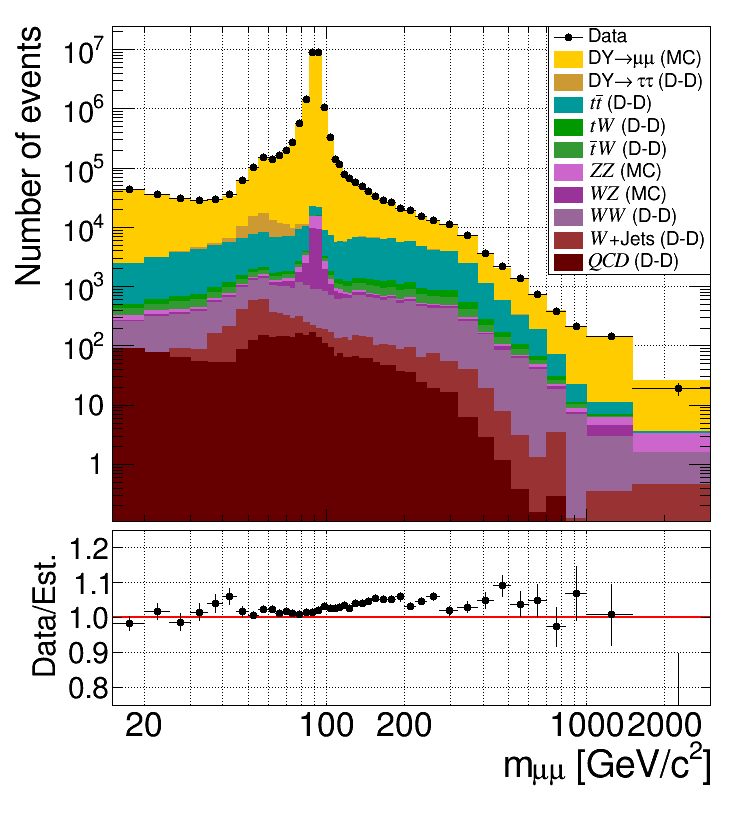
\includegraphics[width=0.5\textwidth]{Kursinis3/Mass_allEst.png}
	\vspace{-0.6cm}
	\caption{\label{fig:MassFinal}
		Eksperimento metu išmatuoto miuonų poros invariantinės masės pasiskirstymo palyginimas su matavimu grįstais
		skirtingų procesų indėlių įverčiais (pažymėta \ltq{m.g.}), išskyrus $\WZ$ ir $\ZZ$ procesų įverčius, kurie
		yra modeliuoti (pažymėta \ltq{MC}) Mėlynos juostos žymi sumines paklaidas.}
\end{figure}


\section{Išvados}
\begin{enumerate}
	\item Šablonų pritaikymo metodas duoda geresnį modeliuotų pasiskirstymų sutapimą su eksperimento metu išmatuotais
	pasiskirstymais nei modeliuotų įvykių normavimas pagal išmatuotą integruotąjį šviesį, todėl manoma, kad šiuo metodu
	įvertinta tikimybė, kad čiurkšlė bus klaidingai atpažintai kaip izoliuotas miuonas, yra teisingesnė.
	\item Su čiurkšlėmis susijusių Drell-Yan proceso triukšmo įvykių skaičiaus įvertis yra labai jautrus
	fizikinio objekto klaidingo atpažinimo tikimybės įvertinimo tikslumui, todėl įverčio sisteminė paklaida yra didelė.
	\item Modeliuoti $\WJets$ ir $\QCD$ procesų įverčiai yra labai prastos kokybės dėl didelio šių procesų reakcijos
	skerspjūvio ir itin mažos tikimybės, kad su jais susiję įvykiai praeis Drell-Yan proceso atranką.
	\item Nors klaidingo atpažinimo metodu įvertintas $\WJets$ ir $\QCD$ procesų indėlis į miuonų poros invariantinės masės
	pasiskirstymą turi nemažus neapibrėžtumus, šio įverčio kokybė yra žymiai geresnė nei modeliuoto, tad fizikinio
	objekto klaidingo atpažinimo metodo taikymas buvo naudingas.
	\item Triukšmo įvykių skaičiaus įvertinimas fizikinio objekto klaidingo atpažinimo metodu pagerino eksperimento
	metu išmatuoto miuonų poros invariantinės masės pasiskirstymo sutapimą su skirtingų procesų įverčiais.
\end{enumerate}


\vspace{2cm}
\addcontentsline{toc}{section}{6 \hspace{0.1cm} Naudotos literatūros sąrašas}
\bibliography{KursinisDarbas}
\bibliographystyle{unsrt}


\section*{Santrauka}
\addcontentsline{toc}{section}{Santrauka}
Viena iš galimų reakcijų didelės energijos protonų susidūrimo metu yra kvarko-antikvarko anihiliacija, kurios
produktas -- leptono ir antileptono pora.
Tokia reakcija yra vadinama Drell-Yan procesu.
Eksperimentinis šio proceso tyrimas pasitarnauja protono sandaros aprašymo tikslinimui bei teorinių modelių testavimui.
Tirdami Drell-Yan procesą eksperimentatoriai ieško leptono-antileptono porų, tačiau jos gali susidaryti ne vien
Drell-Yan proceso metu.
Tokie pašaliniai įvykiai vadinami triukšmo įvykiais ir į jų indėlį svarbu atsižvelgti.
Galimi ir tokie triukšmo įvykiai, kuriuose susidariusios hadronų čiurkšlės yra klaidingai atpažįstamos kaip leptonai.

Šiame darbe pristatomas Drell-Yan proceso triukšmo įvykių skaičiaus įvertinimas fizikinio objekto klaidingo
atpažinimo metodu.
Darbas buvo atliktas analizuojant CERN CMS eksperimento 2016 metais užregistruotus
$13$~TeV energijos protonų susidūrimų duomenis, atitinkančius $35.9$~\invfb integruotąjį šviesį.
Duomenų interpretavimui buvo pasitelkiami CMS kolektyvo paruošti modeliuoti protonų susidūrimų duomenų rinkiniai.
Drell-Yan proceso įvykių atranką praėjusiems miuonams buvo pritaikytos skersinio impulso matavimo skalės pataisos.
Modeliuotiems įvykiams buvo pritaikytas rinkinys pataisų, įskaitančių įvairius neatitikimus tarp eksperimento
ir modeliavimo sąlygų.

Įvykdžius į Drell-Yan procesą panašių įvykių atranką buvo bandoma nustatyti, koks yra triukšmo įvykių, kuriuose
viena ar kelios čiurkšlės buvo klaidingai atpažintos kaip miuonai, skaičius.
Buvo įvertinta čiurkšlės klaidingo atpažinimo izoliuotu miuonu tikimybė.
Šios tikimybės vertės buvo panaudotos įvertinant, kiek $\WJets$ (vienos čiurkšlės) ir $\QCD$ (kelių čiurkšlių)
įvykių galėjo praeiti Drell-Yan proceso įvykių atranką bei koks šių procesų indėlis į eksperimento metu
išmatuotą miuonų poros invariantinės masės pasiskirstymą.
Nustatyta, jog su čiurkšlėmis susiję įvykiai sudaro $0.03\%$ visų Drell-Yan proceso atranką praėjusių įvykių.

\end{document}